\documentclass[11pt, english]{article}
%\usepackage[latin1]{inputenc}
\usepackage[T1]{fontenc}
\usepackage[utf8]{inputenc}
\usepackage[english]{babel}   % S P R A A K


% \usepackage{graphicx}    % postscript graphics
\usepackage{amssymb, amsmath, amsthm, amssymb} % symboler, osv
\usepackage{mathrsfs}
\usepackage{url}
\usepackage{thmtools}
\usepackage{enumerate}  % lister $  
\usepackage{float}
\usepackage{tikz}
\usepackage[all]{xy}   % for comm.diagram
\usepackage{wrapfig} % for float right
\usepackage{hyperref}
\usepackage{mystyle} % stilfilen      
%%   
% one third of the Moebius Strip
%: \strip{<angle>}
\newcommand{\strip}[1]{%
\shadedraw[very thick,top color=white,bottom color=gray,rotate=#1]
 (0:2.8453) ++ (-30:1.5359) arc (60:0:2)
 -- ++  (90:5) arc (0:60:2) -- ++ (150:3) arc (60:120:2)
 -- ++ (210:5) arc (120:60:2) -- cycle;}

%: \MoebiusStrip{<text1>}{<text2>}{<text3>}
\newcommand{\MoebiusStrip}[3]{%
\begin{scope} [transform shape]
    \strip{0}
    \strip{120}
    \strip{-120}
    \draw (-60:3.5) node[scale=6,rotate=30] {#1};
    \draw (180:3.5) node[scale=4,rotate=-90]{#3};
    % redraw the first strip after clipping
    \clip (-1.4,2.4)--(-.3,6.1)--(1.3,6.1)--(5.3,3.7)--(5.3,-2.7)--cycle;
    \strip{0}
    \draw (60:3.5) node [gray,xscale=-4,yscale=4,rotate=30]{#2};
\end{scope}}
%%

\title{Manifolds 2014}
\author{JAC / FM}
\date{}
\begin{document}
\maketitle
\tableofcontents 
\section{Introduction; topological manifolds}

Manifolds are geometric objects that locally look like some $\R^n$ for some natural number $n$. In that respect, they are very easy to understand. The interesting things happen when we glue several pieces of $\R^n$ together.

In Calculus, manifolds (in those rare occasions they were encountered) usually appeared embedded in some larger $\R^n$ or $\C^n$. This is not the path we're going to take - for us, manifolds will be objects in their own right, existing independently of some ``ambient'' space. The way to do this is, exactly, glueing.

We start with the definition of a \emph{topological manifold}.

\begin{defi}
A \emph{topological manifold} $M$ is a topological space such that each $x \in M$ has a neighbourhood $U$ such that $U$ is homeomorphic to $\R^n$.
\end{defi}

Here are some examples of manifolds.

\begin{example}
Setting $M=\R^n$, set $U=\R^n$ for all $x \in M$.
\end{example}

\begin{example}
Any open ball $B$ in $\R^n$: If $x \in B$, let $U=B$. Then I claim that $U \approx \R^n$: just use the map $\vec x \mapsto \frac{1}{1-|\vec x |} \vec x$.
\end{example}

\begin{example}
By the previous example, it follows that any open $U \subseteq \R^n$ is a manifold, by definition of an open set as a union of balls.
\end{example}

\begin{example}
Similarly, any open subset of a manifold is a manifold.
\end{example}

\begin{example}
Up to homeomorphism, there are only two $1$-dimensional manifolds. Namely, the circle $S^1$ and the real line $\R$. The first is compact, the other is not.
\end{example}

\begin{example}
By stereographic projection, every $n$-sphere can be covered by two sheets homeomorphic to $\R^n$. See Figure \ref{stereographic}.
\begin{figure}[th]
\centering
\includegraphics[width=90mm]{stereographic.jpg}
\caption{Stereographic projection.}
\label{stereographic}
\end{figure}
\end{example}

\begin{example}
The $\aleph_0$ number of compact surfaces. These are $2$-spheres attached with $n$ handles, for some natural number $n$.
\end{example}

\begin{example}
The \emph{non-orientable} manifolds. An example of a non-orientable manifold is the Möbius band in Figure \ref{mobius} with the boundary removed. If we keep the boundary, the figure is an example of a \emph{manifold with boundary}.

\begin{figure}[h]
\begin{center}
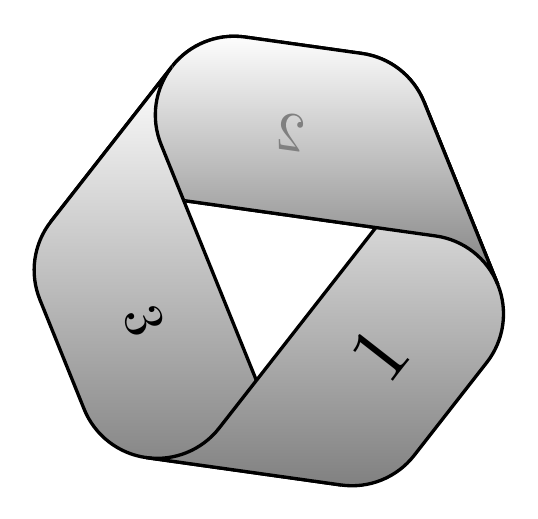
\begin{tikzpicture} [rotate=22,scale=0.5]
  \MoebiusStrip{1}{2}{3}
\end{tikzpicture}
\end{center}
\caption{The Möbius band.}
\label{mobius}
\end{figure}

\end{example}

\begin{example}
The last example (for now) is the projective plane over the reals, called $\PP _\R ^2$. By definition, as a set, it is the set of lines through the origin in $\R^3$. However, it has a nice manifold structure. First, note that a line through the origin in $\R^3$ is determined by giving a point on the $2$-sphere $S^2$. This point is however not unique: the antipodal point gives the same line. This means that we can identify $\PP_\R^2$ with thw quotient space $S^2 / \sim$ where $x \sim -x$. We now give the quotient the quotient topology.

This is not completely enlightening though. There is no obvious local homeomorphisms with $\R^2$, nor do we really have a picture of how $\PP_\R^2$ looks like. The second problem can be solved like this: Note that any line not in the plane $z=0$, has a \emph{unique} representative in the open north hemisphere. Similarly, every line in the plane $z=0$, but with $y \neq 0$, has a unique representative on the equator minus a point. Thus $\PP_\R^2$ can be written as the union of a three cells, namely a $B_2$ (a $2$-ball), a $B_1$ and a $B_0$. So $\PP_\R^2 = B_2 \cup B_1 \cup B_0$, but glued in a special way. We can think of this glueing as ``adding points/lines at infinity''.

There is a natural choice of coordinates on $\PP_\R^2$. We define \emph{homogeneous coordinates}: a point $P$ can be represented by a $3$-tuple $[x_0:x_1:x_2]$, and this tuple is unique up to multiplication by $\R \bs \{ 0\}$. In other words, every point has a representative of the form $[x_0:x_1:x_2]$, where $[x_0:x_1:x_2]=[\lambda x_0:\lambda x_1:\lambda x_2]$. Define the ``basic open sets $U_i$'' as $U_i:= \{ P \in \PP_\R^2 \, | \, x_i \neq 0 \}$. There is a natural bijection between $U_0$, say, and $\R^2$. In $U_0$, every point has a \emph{unique} representative of the form $[1:x_1:x_2]$, and this can be mapped to $(x_1,x_2) \in \R^2$. Now it is an \textbf{exercise} to show that the set $U_i$ is open in the quotient topology.

It is easy to see that the $U_i$ cover $\PP_\R^2$, and so this defined the structure of a topological manifold on $\PP_\R^2$.
\end{example}


\begin{figure}[h]
\begin{center}
\includegraphics[scale=0.5]{connected}
\end{center}
\caption{The connected sum of two tori.}
\label{fig:connected}
\end{figure}


\begin{example}
\label{connectedsum}
One can make new manifolds from old ones by means of the \emph{connected sum}.

One starts with two manifolds $M$ and $N$, removes an open disk from both of them. The boundary of a disk is a $S^1$, and we can identify the two boundaries by an arbitrary homeomorphism $\varphi:S^1 \to S^1$. We glue to get $M\#N$. See Figure 3.%\ref{fig:connected}.  %%% referer til feil figur i dokumentet???
\end{example}

For the Möbius band example to be a manifold, we have to define a manifold with boundary:
\begin{defi}
Let $M$ be a topological space. We say that $M$ is a \emph{manifold with boundary} if every point of $x$ has a neighbourhood homeomorphic to either $\R^n$ or $H_n:=\{ (x^1,\dotsc,x^n) \, : \, x^n \geq 0 \}$, the upper half-plane.
\end{defi}

We call the $n$ in the definition the \emph{dimension} of the manifold. However, to prove that the dimension is well-defined, reduces to proving that if $\R^n \approx \R^m$, then $m=n$. This is a very non-trivial problem, best proved with tools from algebraic topology, using such tools as homology groups and long exact sequences.

\newpage
\section{Differentiable manifolds}

To get a course worth something, one has to have something more than just a topological manifold. We do this by adding structure to $M$, thereby defining the notion of a \emph{differentiable} manifold.

Given two open subsets $U,V$ of $M$ and homeomorphisms $x:U \to x(U) \subseteq \R^n$ and $y:V \to y(V) \subseteq \R^n$, one has transition maps on the intersection $U \cap V$:
\[
\xymatrix{
 U \cap V \ar[d]_x \ar[r]^-y & y(U \cap V)  \subseteq \R^n \\
\R^n \supseteq  x(U \cap V) \ar[ur]^{x \circ y^{-1}}
}
\]
We say that the two charts $(x,U)$ and $(y,V)$ are \emph{$C^\infty$-related} if the map $x \circ y^{-1}$ and the map $y \circ x^{-1}$ are $C^\infty$-maps as maps between subsets of $\R^n$.

Furthermore, we say that a set of charts $\{ (x_i, U_i)\}_{i \in I}$ is an \emph{$C^\infty$-atlas} for $M$ if all the $x_i,x_j$ are $C^\infty$-related and the union $\bigcup_i U_i$ cover $M$.

Here a uniqueness result:

\begin{lemma}
Given an atlas $\mathscr{A}$ on $M$, there exists a unique maximal atlas $\mathscr{A}^\prime$ containing $\mathscr A$.
\end{lemma}
\begin{proof}
Define $\mathscr A$ to be the set of all charts $y$ which are $C^\infty$-related to all charts $x \in A$. Then $\mathscr A$ contains two types of charts: those who belonged to $\mathscr A$, and possibly new ones. Every two charts in $\mathscr A$ are $C^\infty$-related, by definition of atlas, and every pair with one in each are $C^\infty$-related by definition of $\mathscr A^\prime$. Further, evert pair of charts with both in $\mathscr A^\prime$ are $C^\infty$-related: one can intersect their domains with a chart in $\mathscr A$, compose, and conclude.

Clearly $\mathscr A^\prime$ is the unique maximal atlas containing $\mathscr A$.
\end{proof}

Thus:

\begin{defi}
A \emph{differentiable manifold} is a pair $(M,\mathscr A)$, where $M$ is a topological manifold, and $\mathscr A$ is a maximal atlas (of $C^\infty$-related transition functions).
\end{defi}

From now on, when we say ``manifold'', we will always mean ``differentiable manifold''. Note that it is defined as a \emph{pair}, and we cannot forget the atlas, because there are, famously, homeomorphic topological manifolds with different differentiable structures (for example, Milnor's ``exotic spheres'', the first one being the $28$ different differentiable structures on $S^7$).

Here's an example (and probably the only explicit calculation we will do in the course):

\begin{example}
Recall that $S^2$ (the zero set of the equation $x_1^2+x_2^2+x_3^2=1$ in $\R^3$) can be covered by two charts, by stereographic projection (see Figure \ref{stereographic}), by first projecting from the north pole, and then from the south pole. Call these maps $\varphi$ and $\psi$, respectively. We are going to compute the transition maps, to verify that this atlas is actually a $C^\infty$-atlas.

We need to find explicit formulae for $\varphi$ and $\psi$. The first map has domain $\S^2 \bs \{ N \}$ and image $\R^2$. But we want to compute $\psi \circ \varphi^{-1}$, so we start with a point $(a,b)$ in the plane $\R^2$ (embedded in $\R^3$ by $z=0$). We want to connect it with the north pole $(0,0,1)$ by a line, and compute its intersection with the $2$-sphere. The line is given parametrically as \[t(a,b,0)+(1-t)(0,0,1)=(at,bt,1-t).\]
To find the intersection with the sphere, we must compute when the right hand side has norm $1$:
\[
a^2 t^2+b^2 t^2+1-2t+t^2 = 1
\]
Getting rid of the $1$ and cancelling the $t$, we end up with the condition
\[
t = \frac{2}{1+\| a \|},
\]
where $\| a \| = \sqrt{a^2 + b^2}$. In other words, explicitly, we have
\[
\varphi^{-1}(a,b) = \left(\frac{2a}{1+\|a\|},\frac{2b}{1+\|a\|},\frac{\|a \| -1}{1+\|a\|}\right).
\]

To compute $\psi$, one start with a point on the sphere, and find a formula for the the intersection with the $x,y$-plane. So let $(x,y,z)$ be on the sphere. Then $\psi(x,y,z)$ is on the line from $S$ (the south pole) to the plane $z=0$. This line is parametrically given by
\[
t(x,y,z) +(1-t)(0,0,-1) = (tx,ty,tz-1+t).
\]
The $z$-coordinate is zero when $t=\frac{1}{z+1}$. Thus
\[
\psi(x,y,z) = \left( \frac{x}{z+1}, \frac{y}{z+1} \right)
\]

Finally, we can compute the composition $\psi \circ \varphi^{-1}$:

\begin{align*}
\psi \circ \varphi^{-1}(a,b) &= \psi\left(\frac{2a}{1+\|a\|},\frac{2b}{1+\|a\|},\frac{\|a \| -1}{1+\|a\|}\right) \\
&= \left (\frac{2a}{1+\| a \|} \big / \frac{2 \| a \|}{1+\| a \|},\frac{2b}{1+\| a \|} \big / \frac{2 \| a \|}{1+\| a \|}   \right) \\
&= \left ( \frac{a}{\| a \|} , \frac{b}{\| a \|}\right).
\end{align*}

So the transition maps are just inversion about the origin in the $(a,b)$-plane. These are clearly $C^\infty$ functions.
\end{example}

The moral of the story is that we could just as well defined $S^2$ as two copies of $\R^2 \bs \{ 0\}$ glued together with the inversion map, because that's exactly how the differentiable structure is defined, and that is all we care about.

Here's another example:

\begin{example}
Recall that we could write the projective plane $\PP_\R^2$ as the union of three open sets $U_i$, defined by the non-vanishing of one of the homogeneous coordinates. Here one computes (easily) that the transition maps $\varphi_1 \circ \varphi_0^{-1}:\R^2_{(a,b)} \bs \{ a = 0 \}  \to \R^2_{(a,b)} \bs \{ a = 0\}$ are given by \[(a,b) \mapsto \left (\frac{1}{a}, \frac{b}{a} \right).\]
\end{example}

It is time to define \emph{maps} between them.

\begin{defi}
Let $M^n,N^m$ be manifolds (of dimension $n,m$, respectively), and let $f:M \to N$ be a continous map between them. We say that $f$ is \emph{differentiable at $p$} if for all charts $(x,U)$ with $p \in U$ and for all charts $(y,V)$ with $f(p) \in V$, the function $y \circ \restr fU \circ x^{-1}$ is differentiable (as a function between open subsets of $\R^n$ and $\R^m$).
\[
\xymatrix{
 & U \ar[r]^{f_{|U}} & V \ar[dr]^y \\
x(U) \ar[ur]^{x^{-1}} \ar[rrr]_{y \circ f \circ x^{-1}}  & && y(V)
}
\]
If $f$ is differentiable at all points $p \in M$, then we say that $f$ is \emph{differentiable}.
\end{defi}

Thus we have a category $\Diff$ of differentiable manifolds. Its objects are the differentiable manifolds and the maps are differentiable maps. This gives us at once the notion of an \emph{isomorphism} of manifolds: it is just a pair of differentiable maps that compose to the identity in each direction.

We want to define some properties of maps in $\Diff$. To start off, we introduce some notation. Let $f:\R^n\to\R$ be differentiable map, then we define
\[
D_i (f)(a) = \lim_{h \to 0} \frac{f(a^1,\dotsc, a^i + h,\dotsc, a^n)}{h}.
\]

This is nothing but the $i$'th partial derivative. The reason we're not using the usual Leibniz notation is because we want to reserve it for something else. Having established the $D_i$ notation, one recalls the chain rule: Given two maps $g:\R^m \to \R^n$ and $f:\R^n \to \R$, the $D_j$ of the composite is given as
\[
D_j(f \circ g)(a) = \sum_{i=1}^n  D_i\left(f \circ g\right)(f(g(a))) \cdot D_j(g^i)(a)
\]

The classical Leibniz notation will be reserved for tangent fields on manifolds. So let $f:M \to \R$ be a map from a manifold to the real line, and let $(x,U)$ be a chart, and let $p \in U$. Then we define
\[
\frac{\partial f}{\partial  x^i} (p) = \restr{\frac{\partial f}{\partial x^i}}p := D_i(f \circ x^{-1})(x(p))
\]

Thus $\restr{\frac{\partial f}{\partial x^i}}p$ measures the rate of change of the function $f:M \to \R$ \emph{with respect to} the coordinate system $(x,U)$.

Thus we may ask: what happens if we change charts?
\begin{prop}
Let $f:M \to \R$ be a map and let $(x,U),(y,V)$ be two overlapping coordinate charts. Then
\[
\dd{f}{y^i} = \sum_{j=1}^n \dd f{x^j} \dd{x^j}{y^i}.
\]
Or in matrix notation:
\[
\begin{bmatrix}
\dd f{y^i}
\end{bmatrix}_{i=1\dotsc n} = \begin{bmatrix} \dd{x^j}{y^i} \end{bmatrix}_{i=1\dotsc n, j=1\dotsc n} \begin{bmatrix} \dd f {x^j} \end{bmatrix}_{i=1 \dotsc n}.
\]
\end{prop}
\begin{proof}
This is a definition-chase and the chain rule. Explicitly, by definition:
\begin{align*}
 \restr{\dd{f}{y^i}}{p} &= D_i(f \circ y^{-1})(y(p)) = D_i((f \circ x^{-1}) \circ (x \circ y^{-1}))(y(p)) \\
&= \sum
_{j=1}^n D_j(f \circ x^{-1})(x(p)) D_i((x \circ y^{-1})^j)(y(p)) \\
&= \sum_{j=1}^n \restr{\dd{f}{x^j}}{p} \cdot  \restr{\dd{x^j}{y^i}}{p}
\end{align*}
The chain rule appear in the middle.
\end{proof}
\begin{remark}
From now on, all maps will be differentiable, unless otherwise stated. Thus, when referring to a ``map'' above, it should be read as ``differentiable map'' (or better, ``a map in the category $\Diff$'').
\end{remark}

Let $f:M \to N$ be a map of manifolds, and let $(x,U),(y,V)$ be charts on $M,N$, respectively. One can define the \emph{Jacobian matrix of $f$ at $p$} (if $p \in U$):
\[
J_f(p) := \left[ \restr{\dd{(y^i \circ f)}{x^j}}p \right].
\]
Then we define the \emph{rank} of $f:M \to N$ to be the rank of the Jacobian matrix.

\begin{prop}
The rank is well-defined.
\end{prop}
\begin{proof}
Suppose $(x^\prime,U^\prime)$ is another chart containing $p$, and $(y^\prime,V^\prime)$ is another chart containing $f(p)$. Then by restricting both $x$ and $x^\prime$ to $U \cap U^\prime$, we can assume that $U=U^\prime$ and $V=V^\prime$. Then the rank of $f$ at $p$ is both the rank of the Jacobian
\[
\left[ \restr{\dd{(y^i \circ f)}{x^j}}p \right]
\]
and the Jacobian
\[
\left[ \restr{\dd{((y^\prime)^i \circ f)}{(x^\prime)^j}}p \right].
\]
Consider the diagram:
\[
\xymatrix{
& M \ar[r]^f & N \\
& \ar[dl]_{x^\prime} U \ar@{^(->}[u] \ar[d]^x \ar[r]^{\restr fU} & V \ar@{^(->}[u] \ar[d]_y  \ar[dr]^{y^\prime}\\
\R^n \ar[r]_{x \circ x^{\prime -1}} & \R^n \ar[r]^{y \circ f \circ x^{-1}} & \R^n & \ar[l]^{y \circ y^{\prime -1}}\R^n
}
\]
Then $xx^{\prime -1}$, $yfx^{-1}$, and $y y^{\prime -1}$ are maps from (open subsets of) $\R^n$ to $\R^n$. Consider the composition $(y^\prime y^{-1}) \circ (yfx^{-1}) \circ (xx^{\prime -1})=y^\prime f x^{\prime -1}$. Applying the chain rule, we get that the second Jacobian matrix is just a conjugate of the first Jacobian by invertible matrices. These have the same rank.
\end{proof}

We say that a point $p \in M$ is \emph{critical for $f$} if $\rank f < m$ (the dimension of $N$). Otherwise it is \emph{regular}. We say that a point $q \in N$ is regular if all the points in the preimage $f^{-1}(q)$ are regular points.

\begin{example}
Let $M=N=\R$ and let $f:M \to N$. Then a point $p \in \R$ is regular if and only if $f^\prime(p) \neq 0$. In other words, critical points correspond to either maxima, minima or plateaus of the graph of $f$ inside $\R^2$.

One can also think of critical points as points where the inverse function theorem fails (which is the topic of the next lecture). See Figure \ref{criticalpoints}. %%% hmm!!!!
\end{example}

\begin{figure}[ht]
\begin{center}
\includegraphics[scale=0.7]{criticalpoints}
\end{center}
\caption{Critical points of the sine function.}
\label{criticalpoints}
\end{figure}

\newpage
\section{Sard's theorem and the Inverse Function Theorem}

Last time we spoke about critical points, i.e. those points where the Jacobian of a map had non-maximal rank (the maximal rank of a map $\R^n \to \R^m$ is $n$). Sard's theorem says that most points $p \in M$ are non-critical (=regular).

Think of the case $f:\R^2 \to \R$. The graph of such a function is a surface in $\R^3$. In this case, the theorem says that the maxima of this function constitute no ``volume''.

To be able to state the theorem, we have to present some definitions, the first one being, that of ``measure $0$''. We start with a subset $A \subset \R^n$. We say that it has \emph{measure 0} if it can be covered by a sequence of (open) rectangles $R_{ab}$ in such a way that
\[
\sum_{i=1}^n \vol(R_{ab}) < \epsilon
\]
for every $\epsilon > 0$. Here's an example:

\begin{example}
Consider the real line $\{ y = 0 \} \subseteq \R^2$. Intuitively, this has zero volume, \emph{as a subset of $\R^2$}. Let $B_{an,{\frac{1}{n^3}}}$ be the rectangle centered at origo with width $n$ and height $\frac{1}{n^3}$.  Since the height is finite, clearly the union of all these rectangles (for $n \in \N$) cover the real line.  The sum of the volumes is
\[
\sum_{i=1}^\infty \frac{a}{n^2} = \frac{a \pi^2}{6},
\]
so choosing $a < \frac{6 \epsilon}{\pi^2}$, gives total volume less than $\epsilon$.
\end{example}

Now, a subset $A$  of a manifold $M$ has \emph{measure 0} if there exists a countable sequence of charts $(x_i, U_i)$  with $A \subseteq \bigcup U_i$ such that each $x_i(A \cap U_i)$ has measure $0$. To see that this notion is well-defined, one turns to Lemma 6 in Spivak, which says that smooth functions take measure 0 sets to measure 0 sets.

Now, Sard's theorem says the following:
\begin{thm}
If $f:M \to N$ is a $C^\infty$-map of $n$-manifolds, and $M$ has at most countably many components (e.g. one), then the critical values of $f$ form a set of measure zero in $N$.
\end{thm}

This, in some sense, is similar to a theorem in algebraic geometry, which says that the smooth points of a variety are dense in the Zariski topology.

We will not prove Sard's theorem here, but just note that it is at least intuitively plausable.


\subsection{The Inverse Function Theorem}

We are used to thinking about the derivative of a function $f:\R^n \to \R^m$ as a linear approximation to $f$ near a point $p$, i.e. a linear map $f:\R^n \to \R^m$. Linear maps live in \emph{vector spaces} and not on manifolds, so we should really think of the derivative as some kind of \emph{functor} taking maps $f:U \to V$ (where $U,V$ are open subsets of $\R^n$ and $\R^m$, respectively) to \emph{vector space maps} $Df(p):T(\R^n) \to T(\R^m)$, where the $T$ means that we are thinking of just the \emph{vector space} $\R^n$.

For a map $f:\R ^n \to \R^m$ and a point $p \in \R^n$, we define the vector space map $Df(p)$ as follows:
\begin{defi}
If it exists, the map $Df(p):T_p(\R^n) \to T_{f(p)}(\R^m)$ is the unique linear map satisfying
\[
\lim_{h \to 0} \frac{|f(a+h)-f(a)-D_pf(h)|}{|h|} = 0
\]
If we choose the standard coordinate systems on $\R^n$ and $\R^m$, then $D_pf(p)$ has a matrix $\left[ D_j f^i (a) \right]$ of partial derivatives (the Jacobian).
\end{defi}

In particular, the chain rule takes a very nice form with this notation. It just says that given two maps, the derivative of the composition is just the composition of the derivatives:
\[
\xymatrix{
\R^n \ar[r]^f \ar@/_/[rr]_{g \circ f} & \R^m \ar[r]^g & \R^p
}
\]
This gives that
\[
\xymatrix{
T_p(\R^n) \ar[r]^{D_pf} \ar@/_/[rr]_{D_p(g \circ f)} & \R^m \ar[r]^{D_{f(p)}g} & \R^p
}
\]
is commutative.

Now we state the inverse function theorem:
\begin{thm}
Suppose $p \in U \subseteq \R^n$ and that $f:U \to \R^n$ is a smooth function. Suppose further that the Jacobian is non-singular at $p$, i.e. that $p$ is a regular value of $f$ (or equivalently that $D_f(p)$ is an isomorphism of vector spaces).

Then there exists a neighbourhood $V$ of $p$ such that $\restr fV$ is invertible and such that $\restr fV^{-1}$ is smooth. Moreover, the following equality holds:
\[
J_{\restr fV^{-1}}(f(p)) = J_f(p)^{-1}.
\]
\end{thm}

In words (that will have meaning later), this says that if the tangent map is an isomorphism at a point $p$, then $f$ is locally a diffeomorphism near $p$. This is a theorem special to differential geometry. Similar situations does not occur in algebraic or complex geometry, because inverse functions are usually not algebraic/complex.


\pagebreak
\section{Rank theorems}

In this lecture we will elaborate on some ``structure theorems'' on maps $f\colon M \to N$, given restrictions on the rank of $f$, the first one being the following:

\begin{thm}
Let $f:M^n\to N^m$ be a map of manifolds.
\begin{enumerate}
\item If $f:M^n \to N^m$ has rank $k$ at $p$, then there charts $(x,U)$ and $(y,V)$ containing $p$ and $f(p)$, respectively, such that
\[
y \circ f \circ x^{-1}(a) = \left(a^1, \dotsc, a^k, \psi^{k+1}(a), \dotsc, \psi^m(a)\right)
\]
for all $a \in U$.
\item If furthermore, $f:M^n \to N^m$ has rank $k$ in a neighbourhood of $p$, then there are charts $(x,U)$ and $(y,V)$ containing $p$ and $f(p)$, respectively, such that
\[
y \circ f \circ x^{-1}(a) = \left( a^1, \dotsc, a^k, 0, \dotsc, 0 \right)
\]
for all $a \in U$.
\end{enumerate}
\end{thm}
\begin{proof}
  \begin{enumerate}
  \item Start by choosing any coordinate system $(u,U^\prime)$ around $p$. Since the rank of the Jacobian $\left[ \restr{\dd{(y^\alpha \circ f)}{u^\beta}}p \right ]$ is $k$ at $p$, there is some $k \times k$-minor that is non-zero. So, after permuting coordinates, we can assume that this minor is the upper-left block of the Jacobian.

We define new local coordinates as follows:
\begin{align*}
x^\alpha &= y^\alpha \circ f  &\text{for } \alpha={1,\dotsc, k} \\
x^r &= u^r &\text{for } r=k+1,\dotsc, n.
\end{align*}

Now consider the change of basis matrix:
\[
\left[ \restr{\dd{x^i}{u^j}}{p} \right] = \begin{bmatrix}
\dd{(y^\alpha \circ f)}{u^\beta}  & \scalebox{1.5}X \\
\scalebox {1.5}0 & \begin{matrix}1 & & \\  & 1 &  \\&  & 1\end{matrix}
\end{bmatrix}
\]
Since the upper corner has determinant non-zero , the whole has determinant non-zero. Hence, by the inverse function theorem, $(x,U)$ is a diffeomorphism in a neighbourhood $U$ of $p$. Thus $x = (x \circ u^{-1}) \circ u$ is a coordinate system near $p$, and in fact it is the coordinate system we want:

\begin{align*}
y \circ f \circ x^{-1}(a^1,\dotsc, a^n) &= y \circ f\left(f^{\alpha,-1}(y^{\alpha,-1}(a^1),\dotsc, u^{r-1}(a^n)\right) \\
&= \left( a^1,\dotsc, a^k,?,\dotsc, ? \right).
\end{align*}
Where the questions marke denote $u^{-1}(a^r)$, which we don't care about. What is important, is that the coordinates have the desired form.
\item
Start by choosing coordinate systems $(x,U)$ and $(v,V^\prime)$ as in 1). Since the rank of $f$ is $k$ in a neighbourhood, the all of the components of the lower right rectangle of the matrix
\[
\left[ \dd{(v^i \circ f)}{x^j} \right] = \begin{bmatrix}
\begin{matrix}1 & & \\  & 1 &  \\&  & 1\end{matrix} & \scalebox{1.5}0 \\
\scalebox {1.5}X & \begin{matrix} D_{k+1}\psi^{k+1} &\dotsb  & D_n\psi^{k+1} \\
\vdots & & \vdots \\
D_{k+1}\psi^m & \dotsb & D_n\psi^m \end{matrix}
\end{bmatrix}
\]
must vanish in a neighbourhood  of $p$. In particular, this means that $\psi$ is a function only of the first $k$ coordinates of $a$, i.e. that it is constant along the last $n-k$ coordinates.

Now define new local coordinates on $N$ by letting
\begin{align*}
y^\alpha &= v^\alpha &\text{for } r=1,\dotsc,k \\
y^r &= v^r - \psi^r \circ ( v^1, \dotsc, v^k) &\text{for } r=k+1,\dotsc, m.
\end{align*}

Notice that the last line makes sense because $\psi$ only depends on the first $k$ coordinates. It is easy to see that the change of base matrix has non-zero Jacobian at $v(q)$, so $(y,V)$ is actually a coordinate system, where $V$ is a neighbourhood of $f(p)$.

Moreover:
\begin{align*}
y \circ f \circ x^{-1} ( a^1, \dotsc, a^n) &= y \circ v^{-1} \circ v \circ f \circ x^{-1}(a^1,\dotsc, a^n) \\
&= y \circ v^{-1}\left(a^1,\dotsc, a^k, \psi^{k+1}(a),\dotsc, \psi^m(a)\right) \\
&= \left( a^1, \dotsc, a^k, 0,\dotsc,0 \right)
\end{align*}
The first equality is by part 1), and the second follows by definition of $y$.
  \end{enumerate}
\end{proof}

Thus if the rank is constant in a neighbourhood, the theorem says that the map locally looks like an inclusion of the first $k$ coordinates in $\R^m$.

If the rank is maximal, the theorem says even more:
\begin{thm}
\begin{enumerate}
\item If $m \leq n$ and $f:M^n \to N^m$ has rank $m$ at $p$, then for any coordinate system $(y,V)$ around $f(p)$, there is some coordinate system $(x,U)$ around $p$ with
\[
y \circ f \circ x^{-1}(a^1,\dotsc, a^n) = \left(a^1,\dotsc, a^m\right).
\]
\item If $n \leq m$ and $f:M^n \to N^m$ has rank $n$ at $p$, then for any coordinate system $(x,U)$ around $p$, there is a coordinate system $(y,V)$ around $f(p)$ with
\[
y \circ f \circ x^{-1}(a^1,\dotsc, a^n) = \left(a^1,\dotsc, a^n,0,\dotsc, 0 \right).
\]
\end{enumerate}
\end{thm}
\begin{proof}
Part 1 is just the previous theorem. So we concentrate on part $2$. [[comes later]]
\end{proof}

\newpage
\section{Embeddings}
\begin{wrapfigure}{r}{0.4\textwidth}
 \vspace{-20pt}
  \begin{center}
    \includegraphics[width=0.3\textwidth]{cusp}
  \end{center}
 \vspace{-20pt}
  \label{cusp}

  \caption{A cusp.}
\end{wrapfigure}

What does it mean to put one manifold into another manifold? It turns out that this isn't completely trivial to define.

First off, we want the embedding to respect the smooth structure in some sense. This is achieved by requiring that the map has full rank everywhere:

\begin{defi}
A map $f:M^n \to N^m$ for $m \geq n$ is an \emph{immersion} if $\rank f = n$ everywhere.
\end{defi}

\begin{example}
Consider the zero set of the equation $y^2=x^3$, or equivalently, the image of the map $f(t)=(t^2,t^3)$. It is injective everywhere, but it is not an immersion, because the rank is zero at the origin (because the derivative is $(2t,3t^2)$ which is zero for $t=0$). See Figure \ref{cusp}.
\end{example}


\begin{figure}[th]
\centering
\includegraphics{node}
\caption{A nodal curve.}
\label{node}
\end{figure}

\begin{example}
Let $\alpha:\R \to \R^2$ be parametrized by $\left(t^2-1,(t^2-1)t\right)$. It is a nodal curve, and its derivative is $\alpha^\prime(t) = \left(2t,3t^2-1\right)$, which is nowhere zero. But it has self-intersections, and we do not want to allow that. See Figure \ref{node}.
\end{example}

\begin{example}
Another example is given by embedding a curve into the torus with irrational slope: $\alpha(t)=\left( e^{i\sqrt{2}t},e^{i\sqrt{2}t}\right)$.

This is an immersion, but the image is \emph{dense} in $S^1 \times S^1$!
\end{example}

These problems ``usually'' vanish with the following definition:
\begin{defi}
An \emph{embedding} is a map that is both an immersion and a homeomorphism onto its image.
\end{defi}
We call the image of an embedding a \emph{submanifold}.
\begin{remark}
This is a sensible definition: it uses both the topological \emph{and} the differentiable structure of the manifolds, whereas the first definition used only the differentiable structure. A similar situation occurs in algebraic geometry, where a closed immersion of schemes is defined not just as a i closed inclusion of the underlying topological spaces, but as a \emph{pair} $(f,f^{\#})$, where the first is a map of topological spaces, and the second is \emph{surjetive} map of sheaves $f^{\#}:f^\ast \OO_Y \to \OO_X$.
\end{remark}

Here's an important result:
\begin{prop}
\label{proprank}
If $f:M \to N$ has constant rank $k$ in a neighbourhood of $f^{-1}(y)$, then $f^{-1}(y)$ is a closed submanifold of $M$.
\end{prop}
\begin{proof}
To give $f^{-1}(y)$ the structure of a manifold, it is enough to give charts and glueing maps. Since $f$ has rank $k$ everywhere in $f^{-1}(y)$, there exists charts $(x,U) \subset M^n$ and $(y,V) \subset N^m$ such that $y \circ f \circ x^{-1} = (x_1,\cdots,x_n) \mapsto (x_1,\cdots,x_k,0,\cdots,0)$.

We may assume that $y(y)=0$, so that $x(U \cap f^{-1}(y)) = \{ x_1 = x_2 = \cdots = x_k =0 \}$. This is an $n-k$-dimensional closed subspace of $U$.
\end{proof}

\begin{example}
Consider Figure \ref{contour}. If we define a map $F:\R^2\to \R$ by $(x,y) \mapsto x^2-y^2$, we get a function whose graph has a saddle point. As long as we're looking at $F^{-1}(a)$ for $a$ non-zero, the inverse image is a hyperbola, which is a smooth (disconnected) manifold. However, when $a=0$, the fiber (i.e. the contour line) is a pair of double lines, which is not even a manifold. The reason is that the rank of $F$ is zero at $(0,0)$.
\begin{figure}[ht]
\begin{center}
\includegraphics[scale=0.7]{contours}
\end{center}
\caption{The countour lines of the function $F(x,y)=x^2-y^2$.}
\label{contour}
\end{figure}
\end{example}

\begin{example}
Let $f:\R^2 \to \R$ be the map $f(x,y)=x^2+y^2-1$. It has constant rank $1$ as long as we're away from the origin. Then the theorem says that $f^{-1}(0)=\{ x^2+y^2=1 \}\approx S^1$ is a closed submanifold av $\R^2$.
\end{example}

\newpage
\section{Bump functions and partitions of unity}

What makes differential geometry ``taste'' differently than complex or algebraic geometry is the existence of ``bump functions''.

\subsection{Useful functions}
Recall that the \emph{support} of a function $f:X \to \R$ is the closure of the set $\{ x \, | \, f(x) \neq 0 \}$.
\begin{example}
The first function is an example of a non-zero function whose Taylor series around any point is zero (thus it is an non-analytical function).
\[
h(x) =
\begin{cases}
  e^{-\frac{1}{x^2}} & x \neq 0 \\
0 & x = 0.
\end{cases}
\]
\begin{center}
  \includegraphics[scale=.9]{hx}
\end{center}
\end{example}

\begin{example}
This is an example of a function whose support is $[-1,1]$, but is zero everywhere else.
\[
j(x) =
\begin{cases}
  e^{-(x-1)^{-2}} \cdot e^{-(x+1)^{-2}} & x \in (-1,1) \\
0 & x \not \in (-1,1)
\end{cases}
\]
\begin{center}
\includegraphics[scale=0.9]{jx} 
\end{center}
Note that this function is, roughly, the same as $h(x-1)\cdot h(x+1)$ inside $(-1,1)$. By composing with a linear change of coordinates, we get a function which is positive on $(0,\delta)$ and $0$ elsewhere.
\end{example}
\begin{example}
  There is a function $l:\R \to \R$ which is zero for $x \leq 0$, strictly increasing on $(0,\delta)$, and equal to $1$ for $x \geq \delta$:
\[
l(x) = \frac{\int_0^x k(x) \mathrm{dx}}{ \int_0^\delta k(x) \mathrm{dx}}.
\]
\begin{center}
  \includegraphics[scale=.9]{lx}
\end{center}
\end{example}

\begin{example}
\label{ex:constant}
  By mirroring the function $l(x)$ from the previous example around $x=\delta+1$, we get a function $f(x)$  which is constantly equal to $1$ on $(\delta,\delta+1)$, and has support $[0,2\delta + 1]$. By affine transformations, the function can be made to be $1$ on any bounded interval $K$ and support on any interval containing $K$.
\end{example}

\begin{example}
There is a function $g:\R^n \to \R$ which is positive on the open square $(-\epsilon, \epsilon) \times \dotsb \times (-\epsilon, \epsilon)$ and zero elsewhere:
\[
g(x) = \prod_{i=1}^n j(x^i/\epsilon).
\]
\end{example}

\begin{example}
Generalizing Example \ref{ex:constant}, by defining $\phi:\R^n \to \R$ as
\[
\phi(x) = \prod_{i=1}^n f(x^i),
\]
we get a function which is constantly equal to one on a closed, bounded square, and has support in a slightly larger square.
\end{example}

The last example can be generalized to general manifolds:
\begin{prop}
\label{prop:suppfunc}
Let $M$ be a smooth manifold and $K$ a compact subset of $M$ and $U$ an open subset containing $K$. Then there exists a smooth function $\beta\colon M \to [0,1]$ that is constant equal to $1$ on $K$ and compact support contained in $U$.
\end{prop}
\begin{proof}
We first do the case $M=\R^n$. In this case, $K$ is compact, so it is closed and bounded. For each $p \in K$, let $U_p$ be an open square of radius $\epsilon_p$ centered at $p$ and contained in $U$. The set of all these $U_p$ is an open cover of $K$, and since $K$ is compact, we can choose finitely many such $p$. By translation, the function in the last example, can be made such that $f_p$ is positive in the interior of $U_p$ and zero outside (so its support is $\bar{U_p}$), and constant $1$ on $K \cap U_p$. Now define the following function:
\[
\beta(x) = 1 - \prod_p \left(1-f_p(x)\right),
\]
where the product ranges over those finitely many $p$ needed to cover $K$. Then, if $x \in K$, $x$ is contained in one of the $U_p \cap K$, hence $\beta(x)=1$. The support is clearly bounded, hence compact.

Now to the general case. If $K$ is contained in a single chart, we are done by the above. If not, $K$ is contained in finitely many charts $(U_i,x_i)$, hence we can find compact sets $K_1,\cdots, K_k$ with $K \subset \bigcup_{i=1}^k K_i$, $K_i \subset U_i$ and $\bigcup_i U_i \subset U$. Let $\phi_i$ be identically $1$ on $K_i$ and zero on $M \bs U_i$. Then define
\[
\beta(x) = 1 - \prod_{i=1}^k (1-\phi_i(x)).
\]
\end{proof}

\subsection{Partition of unity}

Partitions of unity is an extremely important tool, but to define it, we need some technical definitions. To motivate all this, we will note that when we are done, we will be able to prove that any compact manifold can be embedded into real Euclidean space $\R^N$ for some large $N$.

\begin{defi}
  We say that a family $\UU$ of open sets is an \emph{open cover} of $M$ if
\[
\bigcup_{U \in \UU} U = M.
\]
\end{defi}
\begin{defi}
  We say that $\UU^\prime$ is a \emph{refinement} of $\UU$ if for all $U \in \UU^\prime$, there exists some $V \in \OO$ with $U \subseteq V$. 
\end{defi}
\begin{example}
Cover $\R$ with the single open set $\R$, so that $\UU=\{ \R \}$. Now consider the cover given by $\UU^\prime = \{ (-\infty, 1),(-1,\infty) \}$. Then $\UU^\prime$ is a refinement of $\UU$.

Let $\UU^{\prime \prime}=\{ (-2,2), (0,\infty), (-\infty,0) \}$. Then $\UU^{\prime\prime}$ is \emph{not} a refinement of $\UU^\prime$. 
\end{example}

\begin{defi}
  We say that an open cover $\UU$ is \emph{locally finite} if for every $p \in M$, there are only finitely open sets $U$ in $\UU$ with $\{ p \} \cap U \neq \emptyset$.
\end{defi}

\begin{thm}
  If $\UU$ is an open cover of a connected manifold $M$, then there exists a locally finite refinement $\UU^\prime$ of $\UU$. 

Moreover, we can choose these $\UU^\prime$ in such a way that $\UU^\prime \approx \R^n$ as differentiable manifolds.
\end{thm}

\begin{remark}
We skip the proof. Now it's time to note that we are hiding details under carpets: for this theorem to be true, we must assume that $M$ is $\sigma$-compact, meaning that we can write $M$ as a countable union of compact subsets. In particular, this is clearly true if $M$ itself is compact. Note also that all subsets of $\R^n$ have this property.
\end{remark}

\begin{thm}[Shrinking Lemma]
\label{shrinkinglemma}
Let $\UU$ be an open cover of $M$. Then it is possible to choose for each $U \in \UU$ an open set $U^\prime$ with $\bar{U^\prime} \subset U$ in such a way that the new collection $\{ U^\prime \}$ is also an open cover $M$. 
\end{thm}

\begin{remark}
In particular, this new open cover is a refinement of $\UU$. 
\end{remark}

\begin{thm}[Existence of partitions of unity]

Let $\UU$ be an open locally finite cover of a manifold $M$. Then there is a collection of $C^\infty$-functions  $\varphi_U:M \to [0,1]$ for each $U \in \UU$ such that
\begin{enumerate}
\item $\supp \varphi_U \subset U$ for each $U$.
\item $\sum_{U \in \UU} \varphi_U(p) = 1$ for all $p \in M$. (this makes sense because the cover is locally finite!)
\end{enumerate}
\end{thm}


\begin{defi}
  A collection $\{ \varphi_i:M \to [0,1] \}$ is called a \emph{partition of unity} if (1) the collection $\{ p \, | \, \varphi_i(p) \neq 0 \}$ is locally finite and (2) if $\sum_i \varphi_i(p)=1$ for all $p \in M$. 

If for each $i$ there is an $U \in \UU$ such that $\supp \varphi_i \subset U$, then we say that the collection is \emph{subordinate to $\UU$}. 
\end{defi}

So the theorem says that given a locally finite cover $\UU$  of a manifold $M$, there exists a partition of unity subordinate to $\UU$.

\begin{example}
Let $M= \R$ and cover $M$ by $U_1=(-1,\infty)$ and $U_2=(-\infty,1)$. Let $\varphi_1(x) = \frac{l(x+1)}{l(x+1)+l(-x-1)}$. And similarly, $\varphi_2(x) = \frac{l(-x+1)}{l(x+1)+l(-x+1)}$.
\begin{center}
\includegraphics{partition}
\end{center}
Then the partition of unity looks like the graph above. Notice that it sums to $1$ everywhere.
\end{example}

\begin{thm}
  Let $M^n$ be a compact manifold. Then there exists an embedding $f:M \to \R^N$ for some $N$.
\end{thm}
\begin{proof}
By compactness we can choose a finite number of coordinate systems $\{ (x_i,U_i) \}_{i=1,\ldots,k}$, covering $M$. By the Shrinking Lemma \ref{shrinkinglemma}, choose $U_i^\prime \subseteq U_i$, and by Partition of Unity, choose functions $\psi_i\colon M \to [0,1]$ that are $1$ on $\bar{U_i^\prime}$ and have support contained in $U_i$. This can be done by Proposition \ref{prop:suppfunc}.

Define $f:M \to \R^N$, where $N=k(n+1)$, by
\[
f = \left(\psi_1 \cdot x_1, \ldots, \psi_k \cdot x_k, \psi_1,\ldots, \psi_k\right).
\] 
This is an immersion: any point $p \in M$ is contained in some $U_i^\prime$, and on $U_i^\prime$, where $\psi_i=1$, the $N \times n$ Jacobian matrix contains the identity matrix $\left(\dd{x_i^\alpha}{x_i^\beta}\right)$.

The map is also one-one. For suppose that $f(p)=f(q)$. There is some $i$ with $p \in U_i^\prime$. But then $q \in U_i$ since the support of $\psi_i$ is contained in that set. Moreover, $\psi_i \cdot x_i(p)=\psi_i x_i(q)$, so $p=q$, since $x_i$ is $1-1$.
\end{proof}
\begin{remark}
Note that this embedding is highly non-canonical. It contains several layers of choices. The proof begins by \emph{choosing} a finite open cover, and then \emph{choosing} a refinement, and then choosing a partition of unity. None of these choices are natural in any sense.
\end{remark} 


\newpage
\section{The tangent bundle}

Think of a surface $S \subseteq \R^3$ and let $p$ be a point on $S$. Then the tangent plane of $S$ is a linear subspace of $\R^3$. Thus, in the case of embedded manifold, it is easy to assign a ``tangent space'' to each point $p \in S$. However, for general manifolds, we are not given an embedding anywhere. What we want is some rule that assigns to each point $p \in S$ a vector space of the same dimension as $S$, called the ``tangent space''. Also, we want this rule to reflect the global structure of $S$ in a natural way.

More formally, we want a functor from manifolds to vector bundles, such that its restriction to chart domains, the result is just $\R^n$, as a vector space. To carry this out, we first formally introduce the ``tangent space'' of $\R^n$ (or open subsets thereof).

We define $T(\R^n) := \R^n \times \R^n$, and we write its elements as $(p,v)$ or $v_p$, where we think of the left factor as the \emph{manifold} $\R^n$, and the right factor as the \emph{vector space} $\R^n$. Thus, to each \emph{point} $p$ in $\R^n$, we attach a \emph{vector} $v_p$.

Now we have defined the functor $T$ on objects. Now we define it on morphisms, so let $f:\R^n \to \R^m$ be a smooth function. Then we define $Tf:T(\R^n) \to T(\R^m)$ by $Tf(p,v)=(f(p),Df(p)(v))$. By the chain rule, this is really a functor, because if $g:\R^m \to \R^k$ is another smooth function, we have
\begin{align*}
T(g) \circ T(f) (p,v) &= T(g)(f(p),Df(p)(v)) \\
&= \left( g(f(p)) , Dg(f(p))(Df(p)(v))\right) \\
&= \left( g \circ f (p) , D(g \circ f)(v)   \right) \\
&= T(g \circ f).
\end{align*}

To generalize this construction to general manifolds, we need to notion of a \emph{vector bundle}:

\begin{defi}
  A \emph{vector bundle} over $M$ is a map $\pi:E \to M$, where $E$ is a manifold, such that for each $p \in M$, there is an open neighbourhood $U$, and a homeomorphism $e_q:\pi^{-1}(U) \to U \times \R^n$ in such a way that \[\restr{t}{\pi^{-1}(\{q\})}:\pi^{-1}(\{q\}) \to \{q \} \times \R^n\] is a vector space isomorphism for all $q \in U$.

A \emph{map of vector bundles} is just a commutative diagram
\[
\xymatrix{
E_1 \ar[d]_{\pi_1}  \ar[r]^{\tilde f} & E_2 \ar[d]^{\pi_2} \\
B_1 \ar[r]^f  & B_2
}
\]
such that, when restricted to each fiber, the map $\tilde f:\pi_1^{-1}(p) \to \pi_2^{-1}(f(p))$ is a linear map.
\end{defi}

Thus we have a category of vector bundles, which we shall denote by $\VBundles$. We have a natural map $p:\VBundles \to \Diff$ that sends a vector bundle to its base. The fiber $p^{-1}(M)$ is a category, called the category of \emph{vector bundles over $M$}, which we shall often denote by $\VBundles(M)$.

We call a vector bundle $E$ \emph{trivial} if it is isomorphic to $M \times \R^n$ (with the obvious maps).

This really generalizes the $T(\R^n)$ above: it is trivally a vector bundle over $\R^n$, and it is easy to see that it restricts to a sub-vector bundle for any open subset $U \subset \R^n$. 

Requring only that $T(U)=U \times \R^n$ for $U$ an open subset of $\R^n$ and functoriality, there is a unique extension of $T$ from open subsets of $\R^n$ to general manifolds.

\begin{thm}
Let $M$ be a smooth manifold. Then there is a functor $T:\Diff \to \VBundles$ that to each manifold $M$ associates a vector bundle over $M$ in such a way that if $(U,x)$ is a chart domain of $M$, we have $T(U) = U \times \R^n$. 
\end{thm}
\begin{proof}
  Here is a proof sketch. Cover $M$ by open chart domains $(x_i,U_i)$. Each of these are isomorphic to $\R^n$, so we define $\restr{TM}{U_i} := x_i(U_i) \times \R^n$, with the obvious projection map. On the intersections $U_i \cap U_j$ we have a map $x_j \circ x_i^{-1}: \R^n \to \R^n$, and we define
\[
\restr{TM}{U_i \cap U_j} \to \restr{TM}{U_i \cap U_j}
\]
by 
\[
(u,v) \mapsto \left(x_j \circ x_i^{-1}(u), D(x_j \circ x_i^{-1})(u)(v)\right).
\]
That this is well-defined on triple overlaps should follow from the chain rule, and all these glueing maps make $TM$ into a manifold. Local triviality is clear by construction. 
\end{proof}

We call the vector bundle $\pi:TM \to M$ the \emph{tangent bundle} of $M$.

\begin{example}
  Consider the circle $S^1$. It is covered by two open sets $S^1 \bs N$ and $S^2 \bs S$. The map $\phi_1:S^1 \bs N$ is given by $(x,y) \mapsto \frac{x}{1-y}$, and the inverse map is given by $\phi_1^{-1}(x)=\left(\frac{2x}{x^2+1}, \frac{x^2-1}{x^2+1} \right)$. Similarly, $\phi_2(x,y) = \frac{x}{1+y}$, and the inverse is $\phi_2^{-1}(x)=\left( \frac{2x}{x^2+1},-\frac{x^2-1}{x^2+1} \right)$. Thus $T(S^1)$ is covered by two open sets $U = T(R^1)$ and $V=T(R^1)$. The transition map $\phi_{UV}$ is given by $(x,v) \mapsto (\phi_2 \circ \phi_1^{-1}(x), D(\phi_2 \circ \phi_1^{-1})(x)(v))$, which we compute to be
\[
(x,v) \mapsto \left (\frac{1}{x}, -\frac{v}{x^2}\right).
\]
This is well-defined, since $x \in \R \bs \{ 0\}$.

Then I claim that $TS^1 \approx S^1 \times \R^1$, that is, the tangent bundle of the circle is trivial. To do this, we cover the circle with the same open sets as above, so that $S^1$ is covered by the two open sets $U^\prime \times \R$ and $V^\prime \times \R$ with transition maps $\phi_{U^\prime V^\prime}:(x,v) \mapsto (\frac{1}{x}, v)$. This is truly a product, because the second factor does not interact with the first.

An isomorphism $TS^1 \approx S^1 \times \R^1$ is the same thing as maps from the charts from one manifold to the other that agrees on the overlaps. So we define, from $U\times \R$ to $U^\prime \times \R$ a map given by $(x,v) \mapsto (x,v)$, and from $V \times \R $ to $V^\prime \times \R$, a map given by $(x,v) \mapsto \left (x,-\frac{b}{a^2}\right)$. Then the reader can check that the following diagram commutes, and so we have defined a map on manifolds, that is an isomorphism on charts and agrees on overlaps, hence an isomorphism of manifolds:
\[
\xymatrix{
U \times \R \ar@{->}[r]^{\phi_{UV}} \ar@{->}[d]_{(x,v) \mapsto (x,v)} & V \times R \ar@{->}[d]^{(x,v) \mapsto (x,-\frac{b}{a^2})} \\
U^\prime \times \R \ar@{->}[r]_{\phi_{U^\prime V^\prime}} & V^\prime \times \R
}
\]
\end{example}

\begin{example}[The tangent bundle of $S^2$ is not trivial]

It is not hard to see that a $n$-bundle $E \to M$ is trivial if and only if it admits $n$ everywhere linearly independent sections.

Then the non-triviality of $TS^2$ follows from the the Hairy Ball Theorem, which says that every vector field on the sphere must vanish at least somewhere. This in turn follows from the Poincaré-Hopf theorem, which says that
\[
\sum_{i} \mathrm{index}_{x_i}(X) = \chi,
\]
where the left-hand-side is a certain sum ranging over the zeros of the vector field $X$, and the right-hand-side is the Euler characteristic of the sphere, which is two - so $X$ must have at least one zero.
\end{example}

The construction of the tangent space here is the most intuitive one: locally it looks like $U \times \R^n$. However, there are other views one can take. One is to consider points of $TM$ as equivalence classes of curves, as follows: let $[x,v]_p \in T_pM$. Then we say that this corresponds to a curve $x^{-1} \circ \gamma$ where $\gamma$ is a curve in $\R^n$ with $\gamma^\prime(0) = v$ (here $x$ is a coordinate chart). It is not so difficult to see for every vector $v$ in $T_pM$, there is a curve with derivative $v$. Taking equivalence classes resolves uniqueness.

The other view is to consider elements of $T_pM$ to be \emph{derivations}. To define these, let first $\OO_p$ consist of all functions $f:U \to \R$ where $U$ is a neighbourhood of $p$, where we consider $f:U \to \R$ and $g:V \to \R$ to be equal if there is a neighbourhood $W \subset U \cap W$ such that $\restr{f}{W} = \restr{g}{V}$. More formally, $\OO_p$ is really the direct limit $\varinjlim \OO(U)$, where $\OO(U)$ is the sheaf of $C^\infty$ functions $f:U \to \R$.

Then we claim that $T_pM$ can be considered as the set of \emph{derivations} $\ell:\OO_p \to \OO_p$. Formally, a derivation at $p$ is a function from $\OO_p$ to $\OO_p$ that is linear and satisfies the Leibniz rule
\[
\ell(fg)(p) = f(p)\ell(g)(p) + g(p) \ell(f)(p).
\]

To see that derivations actually land in $\OO_p$, we must show the following lemma:
\begin{lemma}
If $f:W \to \R$ and $g:W \to R$ represent the same function in $\OO_p$, and $\ell$ is a derivation, then $\ell(f)=\ell(g)$.
\end{lemma}
\begin{proof}
Cleary we can assume $g=0$. So we need to prove that if $f$ is zero in a neighbourhood of $p$, then $\ell(f)$ is also zero in a neighbourhood of $p$.

Choose a $C^\infty$ function $h:M \to \R$ with $h(p)=1$ and support contained in $f^{-1}(\{ 0\})$. Such a function exists by Proposition \ref{prop:suppfunc}. Let $q \in W$, where $W$ is the smallest neighbourhood of $p$ such that $f \equiv 0$ on $W$.
\[
0 = \ell(0)(q) = \ell(fh)(0) = f(p)\ell(h)(q)+h(p)\ell(f)(q) = 0 + \ell(f)(q).
\]
Thus $\ell(f)(q)=0$ for all $q \in W$, hence $\ell(f)=0$.
\end{proof}

Here's a lemma:
\begin{lemma}
Let $f \in \OO(U)$ \footnote{From now on, unless otherwise stated, the notation $\OO(U)$ will denote the set of $C^\infty$-functions from $U$ to $\R$.} with $f(0)=0$, where $U \subset \R^n$ and $U$ is convex. Then there are $C^\infty$ functions $g_i: U \to \R$ with
\begin{enumerate}
\item $f(x^1,\cdots,x^n) = \sum_{i=1} ^n x^i g_i(x^1,\cdots, x^n)$ for all $x \in U$.
\item $g_i(0) = D_i(f)(0)$.
\end{enumerate}
\end{lemma}
\begin{proof}
 Define a new function $h_x:[0,1] \to \R$ for each $x \in U$ as $h_x(t)=f(tx)$. This makes sense since $U$ is assumed to be convex. Then
\[
f(x)=f(x)-f(0) = \int_0^1 h_x^\prime (t) \d t = \int_0 ^ 1 \sum_{i=1} ^n D_if(tx) x^i \d t.
\]
Therefore we can let $g_i(x)=\int_0^1 D_i f(tx) \d t$. 
\end{proof}

Note that if $(x,U)$ is a chart domain of $M$ around $p$, then $\restr{\dd{}{x^i}}{p}$ is a derivation at $p$. In fact, the derivations $\restr{\dd{}{x^i}}{p}$ span the space of derivations at $p$. 

\begin{thm}
The set of derivations at $p \in M^n$ is an $n$-dimensional vector space. In fact, if $(x,U)$ is a coordinate system around $p$, then
\[
\restr{\dd{}{x^1}}{p}, \cdots, \restr{\dd{}{x^n}}{p}
\]
span this vector space, and any derivation $\ell$ can be written 
\[
\ell = \sum_{i=1}^n \ell(x^i) \cdot \restr{\dd{}{x^i}}{p}.
\]
\end{thm}
\begin{proof}
We can clearly assume $M=\R^n$. Then using the Lemma, we see that any $\ell(f)$, where $\ell$ is a derivation, can be written as
\[
\ell(f) = \sum_{i=1} ^n \ell(x^i) \dd{f}{x^i}(0).
\]
Thus they span the space of derivations, and they are clearly linearly independent. 
\end{proof}

If $(y,V)$ is another coordinate system, then we know that $\restr{\dd{}{y^i}}{p} = \sum_{j=1}^n \restr{\dd{x^j}{y^i}}{p} \restr{\dd{}{x^j}}{p}$, so the derivations transform exactly the same way as the charts of $TM$. So we identify them.


\subsection{Operations on vector fields}


A \emph{vector field} is a section of $TM$. They are often denoted by capital letters such as $X,Y$ and $Z$. The vector $X(p) \in M_p$ is often denoted $X_p$. Thinking of $TM$ as the set of derivations, we have
\[
X(p) = \sum_{i=1}^n a^i(p) \frac{\partial}{\partial x^i} \Big|_p
\]
for some continuous functions $a^i(p)$.

If $X$ and $Y$ are vector fields, then they can be added:
\[
(X+Y)(p) = X(p) + Y(p).
\]
Similarly, if $f: M \to \R$, we can define the vector field $fX$ by
\[
fX(p) = f(p) X(p).
\]

Thus we see that the set of vector fields, $\Gamma(TM)$, is a module over the $C^\infty$-functions $C^\infty(M)=\Gamma(\OO_
M)$.

If $f: M \to \R$ is a function and $X$ is a vector field, then we can define a new function ${X}(f):M \to \R$ by letting $X$ operate on $f$ at each point:
\[
X(f)(p) = X_p(f).
\]

\begin{example}
  Let $M=\R^3$ and let $X$ be the vector field $X= x \dd{}{x} + y \dd{}{y}$. Let $f$ be the function $f(x,y,z)=x^2+y^2+z^2$. Then
\[
X(f) = x \dd{f}{x} + y \dd{f}{y} = 2x^2+2y^2.
\]
\end{example}

\newpage
\section{Tensors}

 \subsection{Miscellany on the exterior algebra}
The construction of the tangent bundle can be generalized to give other types of vector bundles: each fiber $TM_p$ can be dualized to give $T^\ast M_p$, the dual vector space. These spaces glue to give the \emph{cotangent bundle}, denoted by $T^\ast M$. It has a basis consisting of \emph{differentials}.

Now each of the $T^\ast M_p$ are finite-dimensional vector spaces, and as such, we can form the \emph{exterior algebra} $\bigwedge T^\ast M_p$. This is the quotient of the tensor algebra on $T^\ast M_p$ by the two-sided ideal generated by elements of the form $v_1 \otimes \cdots \otimes v_k$ with $v_i=v_{i+1}$ for some $i$.  This is a graded algebra, so we write $\bigwedge T^\ast M_p = \bigoplus_{k=0}^n \bigwedge^k T^\ast M_p$. The sum is finite, since $\bigwedge^{n+1} T^\ast M_p=0$, as is easily seen (here $n$ is the dimension of $M$). Elements of $\bigwedge^p T^\ast M_p$ are called $p$-forms, and we will see later that they are what one integrates over.

Since we have a canonical isomorphism (for vector spaces $V$) $\bigwedge V^\ast \simeq (\bigwedge V)^\ast$, we think of the exterior algebra as parametrizing multilinear maps $T_pM \times \ldots \times T_pM \to \R$.

\subsection{The cotangent bundle}

Given a map $f:M \to \R$, we can produce a section of the cotangent bundle:
\begin{defi}
We define a section $\d f: M \to T^\ast M$ as follows: $\d f(p)$ should act on tangent vectors, so given a tangent vector $X_p \in T_pM$, we define \[
\d f(p) (X_p) := X_p(f)
\]
\end{defi}
To see how this looks like in a chart, see the Appendix.

The cotangent bundle have better functorial properties than the tangent bundle. In the case of the tangent bundle, there were no way to push tangent fields forward nor pull them back via a map $f:M \to N$. However, it is possible to pull back cotangent fields (this is sort of a miracle, as the cotagent bundle does not appear all that different from the tangent bundle). Given a map $f:M \to N$, and a section $\omega:N \to T^\ast N$, we can define a new section $f^\ast \omega:M \to T^\ast M$ as follows: we must say how it acts on vectors $X_p \in T_pM$:
\[
f^\ast \omega(p)(X_p) := \omega(f(p))(f_\ast(X_p)).
\]
The idea is clear: tangent vectors can be pushed forward, and this allows us to act on it by $\omega$.  To see how this works in coordinates, see the Appendix.

Wikipedia has a good article on pullbacks: \url{http://en.wikipedia.org/wiki/Pullback_(differential_geometry)}. 

\begin{example}
Let $M=\R^3$. Let $\omega$ be the section of the cotangent bundle defined by $z \d x-\d z$. Let $X=y \dd{}{x}+x \dd{}{y}$. Then 
\[
\omega(X) = z.
\]
Here we use only that $\d x^i$ and $\dd{}{x^i}$ are dual bases.
\end{example}

\begin{example}
Let $c:S^1 \to \R^2$ be given by $\theta \mapsto (\sin \theta, \cos \theta)$ and let $\omega = y \d x - x \d y$ be a differential form on $\R^2$. Then $c^\ast \omega$ is given by
\[
c^\ast \omega = \cos \theta \dd{c^1}{\theta} \d \theta -\sin \theta \dd{c^2}{\theta} \d \theta
 = \left( \cos^2 \theta + \sin^2 \theta  \right) \d \theta = \d \theta.
\]
\end{example}

\subsection{General tensor fields}

\begin{prop}
The smooth bilinear pairing $\Gamma(TM) \times \Gamma(T^\ast M) \to C^\infty (M)$ given by $(X,\omega) \mapsto \omega(X)$ defines an isomorphism $\Gamma(T^\ast M) \approx \Gamma(TM)^\ast$. 
\end{prop}
Thus to give a tensor field is the same as giving a multilinear map from tangent vectors. This is really a theorem, and relies heavily on the existence of bump functions.
 

\newpage
\section{Vector fields and differential equations}
Let $X: M \to TM$ be a vector field. Then one can ask: is there a curve $\rho:(-\eps,\eps) \to M$ with $\rho(0)=p \in M$ such that
\[
\rho^\prime(t) = X_{\rho(t)} \quad \forall t \in (-\eps,\eps) ?
\]

This is a local question, so we can assume that $M=\R^n$. Then a vector field $X$ on $\R^n$ is a just a smooth function $f:V\to \R^n$, where $V$ is some open neighbourhood, which we assume contains zero. Then the above equation just reads:
\[
\rho^\prime(t) = f(\rho(t)).
\]
This is just an ordinary differential equation of order one. In the beginning of this section we will study the existence and uniqueness of solutions of these in $\R^n$.

Two examples will illuminate the kind of pathologies (or problems, if you like) that can arise:

\begin{example}
Set $n=1$ and $f(y)=-y^2$. We seek a curve $c(t)$ with $c(0)=x \in \R$. Here $f$ corresponds to the vector field $X$ that assigns to every number $y$ a vector pointing backward of length $y^2$. We get the equation
\[
-\frac{1}{c^2} \frac{d c}{d t}= 1.
\]
Integrating both sides:
\begin{align*}
\int -\frac{1}{c^2} \frac{dc}{dt} dt &= \int 1 dt \\
\int -\frac{1}{c^2} dc &= \int 1 dt \\
\frac{1}{c} &=t + C,
\end{align*}
yielding either $c(t)=1/(c+C)$ as a solution, for some constant $C$, or $c(t)=0$ for all $t$, the latter alternative occuring if $c(0)=0$. But if $c(0) \neq 0$, the solution is not defined for all $t$! It does not extend outside $(-\frac{1}{x},\frac{1}{x})$ in both directions. This is one of the problems that can occur.
\end{example}

\begin{example}
Again $n=1$. Now let $f(y)=y^{2/3}$.  Set $c(0)=0$. Then we get the equation
\[
\frac{dc}{dt} = c^{2/3}, \quad c(0)=0.
\]
But there are two solutions! The curve is not unique!
\end{example}

There is a theorem, however:
\begin{thm}
Let $V \subset \R^n$ be open and $f:V \to \R^n$. Let $x_0 \in V$ and $a > 0$ be such that $\bar{B_{2a}(x_0)} \subset V$. If there are $K,L$ such that 
\begin{enumerate}
\item $|f(x)| \leq L$ on $\overline{B_{2a}(x_0)}$, i.e. $f$ is $L$-bounded.
\item $|f(x)-f(y)| \leq K|x-y|$ on $\overline{B_{2a}(x_0)}$, i.e. $f$ is $K$-Lipschitz.
\newcounter{enumTemp}
\setcounter{enumTemp}{\theenumi}
\end{enumerate}
then choose $b > 0$ such that
\begin{enumerate}
\setcounter{enumi}{\theenumTemp}
\item $b \leq 1/L$ and 
\item $b \leq 1/K$. 
\end{enumerate}
Then for each $x \in \overline{B_a(x_0)}$, there exists a unique curve $\alpha_x:(-b,b) \to U$ such that
\[
\alpha_x^\prime(t) = f(\alpha_x(t)) \, \text{ and } \alpha_x(0)=x.
\]
\end{thm}
\begin{proof}[Sketch of proof] Topologize the set of maps $Y= \{ \alpha:(-b,b) \to \overline{B_{2a}(x_0)}\}$ by the sup metric. Then $M$ is a complete metric space. One defines an operator $S:Y\to Y$ by 
\[
(S\alpha)(t) = x + \int_0^t f(\alpha(u)) du.
\]
Then one sees that if $S$ has a fixed point, then it is a solution to our differential equation. One shows that $S$ is a contraction, and this implies that there exists a unique fixed point solution by the contraction lemma of analysis.

Then there is some checking to do, and the proof is complete.
\end{proof}

Write $\alpha_x(t)$ as $\alpha(t,x)$ to get a map
\[
\xymatrix@R=3pt{
\alpha:(-b,b) \times \overline{B_a(x_0)} \ar[r] & V \\
(t, x ) \ar@{|->}[r] & \alpha(t,x)=\alpha_x(t)
}
\]
satisfying $\alpha(0,x)=x$ and $\frac{d}{dt} \alpha(t,x) = f(\alpha(t,x))$. This map $\alpha$ is called the \textbf{local flow} for $f$ in $(-b,b) \times B_a(x_0)$.

Suppose $y=\alpha_x(t_0)$ for some $t_0 \in (-b,b)$ (think of this as starting at $x$ and following the flow for a time $t_0$). Then the reparametrized integral curve
\[
\xymatrix@R=3pt{
t \ar@{|->}[r] & \beta(t) := \alpha_x(t+t_0)
}
\]
satisfies $\beta^\prime(t)= f(\alpha(t_0+t))=f(\beta(t))$, with $\beta(0)=\alpha_x(t_0)=y$. This means that $\beta$ satisfies the conditions that uniquely determine $\alpha_y$, so $\beta(t)=\alpha_y(t)$ for $t$ near $0$ on 
\[
(-b,b) \cap (-b-t_0, b-t_0).
\]
This means that $\alpha_x(t+t_0)=\alpha_y(t)$ for $t$ near zero. Thus:
\begin{prop}
For each $t \in (-b,b)$ we get a map
\[
\xymatrix@R=3pt{
\phi_t:B_a(x_0) \ar[r]& V \\
x \ar@{|->}[r] & \alpha(t,x)
}
\]
Such that $\phi_0(x)=x$ and $\phi_{s+t}(x)=\phi_s(\phi_t(x))$ for $s,t,s+t \in (-b,b)$. In particular, $\phi_{-t}=\phi_t^{-1}$, so each $\phi_t$ is a bijection.
\end{prop}

\begin{thm}
The flow
\[
\xymatrix@R=3pt{
\alpha:(-b,b) \times B_a(x_0) \ar[r] &  V
}
\]
is continous. Hence each $\phi_t$ is also continous. 
\end{thm}
\begin{proof}[Sketch of proof]
Let $S$ denote the operator used in the previous theorem. Using a geometric series trick, one proves that 
\[
\sup_t |\alpha(t,x)-\alpha(t,y)| = \| \alpha_x - \alpha_y \| \leq \frac{1}{1-bK} |x-y|,
\]
where $\alpha_x$ is a solution of the differential equation starting at $x$ and $\alpha_y$ a solution starting at $y$. This inequality implies continuity of $\alpha$.
\end{proof}

\begin{prop}[Spivak cites Lang]
If $f: V \to \R^n$ is $C^\infty$, then the flow is also $C^\infty$. Hence each $\phi_t$ is smooth.
\end{prop}
\begin{proof}"Introduction to Differentiable Manifolds" by Serge Lang.
\end{proof}


Here's a theorem:
\begin{thm}
Let $X$ be a $C^\infty$ vector field on $M$ and let $p \in M$. Then there is an open set $V$ containing $p$ and an $\epsilon > 0$ such that there is a unique collection of diffeomorphisms $\phi_t: V \to \phi_t(V) \subset M$ for $|t| < \epsilon$ with the following properties:
\begin{enumerate}
\item $\phi:(-\epsilon,\epsilon) \X V \to M$ defined by $\phi(t,p)=\phi_t(p)$ is $C^\infty$.
\item If $|s|,|t|,|s+t| < \epsilon$, and $q$ and $\phi_t(q) \in V$, then
\[
\phi_{s+t}(q) = \phi_s \circ \phi_t(q).
\]
\item If $q \in V$, then $X_q$ is the tangent vector at $t=0$ of the curve $t \mapsto \phi_t(q)$.
\end{enumerate}
\end{thm}

If $M$ is compact, or more generally, if $X$ has compact support, then the local diffeomorphisms above can be extendend to all of $M$:

\begin{thm}
If $X$ has compact support, then there are diffeomorphisms $\phi_t:M \to M$ for all $t \in \R$, satisfying the above three properties.
\end{thm}

For proof, see Spivak. To get a sense of what this theorem is about, image $X$ being a vector field on the sphere: let imagine it be horizontal ``winds''. Then the $\phi_t$ ``twist'' the sphere more and more.

The map $t \mapsto \phi_t$ above is called a \emph{1-parameter group of diffeomorphisms} and is \emph{generated by $X$}. If $\mathrm{Diff}(M)$ is the group of diffeomorphisms of $M$, then the above tells us that each vector field $X$ gives us a map $\R \to \mathrm{Diff}(M)$, given by $t \mapsto \phi_t$. 

\begin{thm}
  Let $X$ be a smooth vector field on $M$ with $X(p) \neq 0$. Then there is a coordinate system $(x,U)$ around $p$ such that
\[
X = \dd{}{x^1}.
\]
\end{thm}

\subsection{Lie derivatives}

Here are some definitions that are really different instances of the same definition: 
\begin{align*}
  L_Xf &= X(f) = \lim_{h \to 0} \frac 1h \left[ f \circ \phi_h - f \right] \\ 
L_X \omega &= \lim_{h \to 0} \frac 1h \left[ (\phi_h^\ast \omega)-\omega \right] \\
L_XY &= \lim_{h \to 0} \frac 1h \left[ Y-(\phi_{h\ast}Y)_p \right]
\end{align*}

\begin{prop}
Let $X,Y_1,Y_2$ be vector fields and $\omega_1,\omega_2$ be covector fields. Then
\begin{enumerate}
\item $L_x(Y_1 +Y_2) = L_XY_1+L_XY_2$.
\item $L_X(\omega_1+\omega_2)=L_X\omega_1+L_X\omega_2$.
\item $L_X(fY) = Xf \cdot Y + f \cdot L_XY$.
\item $L_X(f \cdot \omega) = Xf \cdot \omega + f \cdot L_X \omega$.
\end{enumerate}
\end{prop}

If we let $[X,Y]$ denote the vector field given by $[X,Y]_p(f)=X_p(Yf)-Y_p(Xf)$, then one sees that
\[
L_XY = [X,Y].
\]

Now it follows, almost trivially, that
\[
L_XY = -L_YX
\]
and
\[
L_XX=0.
\]
We also have the Jacobi identity:
\[
[X,[Y,Z]] + [Y,[Z,X]]+[Z,[X,Y]] = 0.
\]

Recall: If we have a diffeomorphism, we can push forward vector fields by defining $(\alpha_\ast X)_q = \alpha_\ast X_{\alpha^{-1}(q)}$.

\begin{lemma}
 Let $\alpha:M \to N$ be a diffeomorphism and $X$ a vector field on $M$ which generates $\{ \phi_t \}$. Then $\alpha_\ast X$ generated $\{ \alpha \circ \phi_t \circ \alpha^{-1}\}$.
\end{lemma}

\begin{corr}
  If $\alpha:M \to M$, then $\alpha_\ast X = X$ if and only if $\phi_t \circ \alpha = \alpha \circ \phi_t$ for all $t$.
\end{corr}

\begin{lemma}
 Let $X$ generate $\{ \phi_t \}$ and $Y$ generate $\{ \psi_t \}$. Then $[X,Y]=0$ if and only if $\phi_t \circ \psi_s = \psi_s \circ \phi_t$ for all $s,t$.
\end{lemma}

\begin{thm}
 If $X_1,\cdots,X_k$ are linearly independent $C^\infty$ vector fields around $p$ and $[X_i,X_j]=0$ for all $i,j$, then there is a coordinate system $(x,U)$ around $p$ such that
\[
X_\alpha = \dd{}{x^i}
\]
for $i=1,\cdots,n$. 
\end{thm}

\newpage
\section{Differential forms}

Depending upon taste, there are several ways to define differential forms. This has already been mentioned in an earlier chapter. Perhaps this is the time to reflect upon the strange order of things in Spivak's book?

Suffice it to say that the only thing that is needed of the exterior algebra, regardless of the particular construction, is the anticommutativitiy property, mimicking determinants (or if you're so inclined: defining determinants).

\subsection{Basic theorems}

\begin{thm}
 Let $f:M \to N$ be a map between $n$-manifolds of the same dimension $n$. Let $(x,U)$ be a coordinate system around $p \in M$ and $(y,V)$ be a coordinate system around $q=f(p) \in N$. Then
\[
f^\ast(g\,  \d y^1 \wedge \ldots \wedge \d y^n) = (g \circ f) \cdot \det \left( \dd{y^i \circ f}{x^j} \right) \d x^1 \wedge \ldots \wedge \d x^n.
\]
\end{thm}

\begin{thm}
 A manifold $M$ is orientable if and only if there exists a non-vanishing form $\omega \in \Omega^n(M)$. 
\end{thm}

\subsection{The de Rham complex}
If
\[
\omega = \sum_I \omega_I dx^I.
\]
Then we define
\[
\d \omega := \sum_I \d\omega _I \d x^I = \sum_I \sum_{\alpha=1}^n \dd{\omega_I}{x^\alpha} \d x^\alpha \wedge \d x^I .
\]

\begin{example}
Let $\omega$ be the $2$-form on $\R^3$ defined by $\omega = x dx \wedge dy -y \d x \wedge \d z$. Then
\[
\d \omega = \d x \wedge \d x \wedge \d y - \d y \wedge \d x \wedge \d z = \d x \wedge \d y \wedge \d z.
\]
\end{example}

\begin{prop}
\begin{enumerate}
\item $\d (\omega_1 + \omega_ 2 ) = \d \omega_1 + \d \omega_2$.
\item There is a Leibniz rule: if $\omega_1$ is a $k$-form, then
\[
\d (\omega_1 \wedge \omega_2) = \d \omega_1 \wedge \omega_2 + (-1)^k \omega_1 \wedge \d \omega_2.
\]
\item $d^2=0$.
\end{enumerate}
Further, if $d^\prime$ is another function $\Omega^k(M) \to \Omega^{k+1}(M)$ obeying these rules, then $d=d^\prime$. 
\end{prop}

\begin{corr}
There is a unique operator from $k$-forms on $M$ to $k+1$-forms on $M$ satisfying the above rules.
\end{corr}
\begin{proof}
The above proposition says that for each coordinate system $(x,U)$, we have a unique $d_U$ defined. Given the form $\omega$ and $p \in M$, pick any $U$ with $p \in U$ and define
\[
\d \omega(p) = \d (\omega_{U})(p).
\]
This proves the claim. \footnote{However, I don't see why. If $U^\prime$ is another coordinate chart, how does one see that $d_{U^\prime}(\omega |U^\prime)(p)$ gives the same number?}

\end{proof}

\begin{prop}
\label{pullbackcomm}
If $f:M \to N$ is $C^\infty$ and $\omega$ is a $k$-form on $N$, then 
\[
f^\ast (d \omega) = d(f^\ast \omega).
 \]

 \end{prop}

\subsection{The Poincaré Lemma}

Recall that a manifold $M$ is \emph{smoothly contractible to a point $p_0 \in M$} if there is a map $H:M \times [0,1] \to M$ such that $\restr{H}{1}=\id_M$ and $\restr{H}{0}$ is the constant map mapping to $p_0$. 

\begin{example}
The canonical example is $\R^n$: a contraction to $\vec 0 \in \R^n$ is defined just by $t \vec x $. More generally, any convex region in $\R^n$ is contractible. Even more generally, every star-shaped region in $\R^n$ is contractible. 

Even more generally, any region homotopic to a starshaped (hence convex) region is contractible.
\end{example}

The Poincaré Lemma states that if $\omega$ is a closed form on a contractible manifold $M$, then $M$ is exact. In short, $H^k_{dR}(M)=0$ for $k > 0$. In fact, we will prove something more general. To do that, we need some terminology:

For any $t \in [0,1]$ we have natural maps $i_t: M \hookrightarrow M \times [0,1]$. Thus for each $t$, we have pullback maps $i_t^\ast: \Omega_{M \times [0,1]}^k \to \Omega_M^k$. By Proposition \ref{pullbackcomm}, this induces maps on cohomology. We will prove that they in fact define the \emph{same} map on cohomology. In fact, they are chain homotopic. We will construct a map $I:\Omega_{M \times [0,1]}^{k+1} \to \Omega_M^k$ for all $k$, such that $\d (I \omega)+I(\d \omega) = i_1^\ast \omega - i_2^\ast \omega$. By standard homological algebra, this implies that the maps on cohomology are equal.

We have the following diagram:
\[
\xymatrix{
\Omega_M^{k-1} \ar[r]^d & \Omega_M^k & \\
\Omega_{M \times [0,1]}^{k-1} \ar@<-0.5ex>[u]_{i_1^\ast} \ar@<0.5ex>[u]^{i_0^\ast } \ar[r]^d &
\Omega_{M \times[0,1]}^k \ar@<-0.5ex>[u]_{i_1^\ast} \ar@<0.5ex>[u]^{i_0^\ast } \ar[r]^d  \ar[ul]_I &
\Omega_{M \times[0,1]}^{k+1} \ar[ul]_I
}
\]
We want to show the relation $\d(I \omega)+I(\d \omega)=i_1^\ast \omega - i_2^\ast \omega$ for some $I$ that will be defined now.

Recall that if $V$ is a vector space that is the tensor product of two vector spaces $A,B$, then $\bigwedge^k V = \bigoplus_{i+j=k} \bigwedge^i A \otimes \bigwedge^j B$. Applying this to $\Omega_{M \times [0,1]}^k$ gives that we have a canonical decomposition as abelian groups

\[
\Omega_{M \times [0,1]}^k \approx \Omega_M^k \oplus \Omega_{[0,1]}^1 \otimes \Omega_M^{k-1} \approx \Omega_M^k \oplus \Omega_M^{k-1},
\]
where the last isomorphism is non-canonical, and can be seen after choosing bases. In particular, this says that any $k$-form $\omega \in \Omega_{M \times [0,1]}^k$ can be written uniquely (after choosing bases) as $\omega_1 + (\d t \wedge \eta)$ for some $\eta \in \Omega_{M \times [0,1]}^{k-1}$.\footnote{As it stands, this is not precise. There exists a canonical splitting, but not as stated. Both factors are still $C^\infty(M \times [0,1])$-modules, and this is not reflected in the notation.} 

Having written $\omega$ in this way, we define $I$ as follows:
\[
I\omega(p)(X_1,\cdots,X_{k-1}) := \int_0^1 \eta(p,t)(i_{t\ast} X_1,\ldots, i_{t\ast}X_{k-1}) \d t.
\]
In coordinates, this works as follows: Suppose $(x,U)$ is a coordinate chart. Then we can write $\omega= \sum_I a^I dx^I + \sum_J a^J \d t \wedge dx^J$ where $I$ ranges over $k$-subsets of $\{1,\cdots,n\}$, and $J$ ranges over $(k-1)$-subsets of $\{1,\cdots, n\}$. Then $\eta=\sum_J a^J dx^J$. Thus
\[
I\omega(p) = \sum_J \int_0^1 a^J(p,t) \d t \, dx^J.
\]

Here's the theorem:
\begin{thm}
 For any $k$-form $\omega$ on $M \times [0,1]$, we have
\[
i_1^\ast \omega - i_0^\ast \omega = \d (I\omega) + I(\d \omega).
\]
\end{thm}
\begin{proof}
 Since all maps involved are linear, there are basically just two cases. \textbf{Case A} is when $\omega= \omega_1$ (in the notation above), involving no $\d t$-terms, say $\omega = f dx^I$. In this case $I\omega =0$, so we need to prove that $i_1^\ast \omega - i_0^\ast \omega = I(\d \omega)$. The left hand side is just
\[
i_1^\ast \omega(p) - i_0^\ast \omega(p) = f(p,1) dx^I - f(p,0) dx^I=\left(f(p,1)-f(p,0)\right) \d x^I.
\]
The right hand side is
\begin{align*}
I(d(f \d x^I)) &= I\left(\left( \sum_i \dd{f}{x^i} dx^i + \dd{f}{t}\right) \wedge dx^I\right) \\
&=\left( \int_0^1 \dd{f}{t} \d t \right) dx^I
\end{align*}
But these two expressions are equal by the fundamental theorem of calculus.

Now for \textbf{Case B}. Here $\omega = f \d t \wedge \d x^J$. In this case $i_t^\ast \omega = 0$ for all $t$, so we want to prove that $\d (I \omega) = - I(\d \omega)$:
\begin{align*}
\d (I \omega)(p) &= \d \,  \left( \int_0^1 f(p,t) \d t \wedge dx^J \right) \\
&= \sum_{i=1}^n \dd{}{x^i}\left( \int_0^1 f(p,t)\right) \d x^i \wedge dx^J \\
I(\d \omega)(p) &= I\left(\sum_{i=1}^n \dd{f}{x^i} \d x^i \wedge \d t \wedge \d x^J\right) \\
&=I\left( - \sum_{i=1}^n \dd{f}{x^i} \d t \wedge \d x^i \wedge \d x^J\right) \\
&= -\sum_{i=1}^n \left(\int_0^1 \dd{f}{x^i} \d t \right) \d x^i \wedge \d x^J.
\end{align*}
Thus the proof is complete.
\end{proof}

The Poincaré Lemma now follows as an easy corollary:
\begin{lemma}[Poincaré\footnote{Though it is not clear if Poincaré actually proved it.}]

If $M$ is contractible, then $H^k_{dR}(M)=0$ for $k > 0$. 
\end{lemma}

\begin{proof}
Let $\omega$ be such that $d \omega =0$.  We are given a $H:M \times [0,1] \to M$ as above. I.e. such that $H \circ i_0 = p_0$ (the constant map to $p_0$), and $H \circ i_1 = \id_M$. Thus \[\omega = \id_M^\ast \omega = (H \circ i_1)^\ast \omega = i_1^\ast (H^\ast \omega) \] and also \[ 0 = (H \circ i_0)^\ast(\omega) = i_0^\ast (H^\ast \omega)\] 
This last pullback is zero because every form on a point-space vanishes. But also $\d (H^\ast \omega) = H^\ast( \d \omega)=H^\ast(0)=0$, by Proposition \ref{pullbackcomm}. 
But then $\omega = i_1^\ast(H^\ast \omega) = d(I(H^\ast \omega))$ by the Theorem. Thus $\omega$ is a boundary, and so $H^k=0$. 
\end{proof}


\newpage
\section{Integration}

A map $c:[0,1]^k \to M$ is called a \emph{singular $k$-cube} in $M$. By convention, a singular $0$-cube is just the assignment of a point in $M$. The inclusion map $I:[0,1]^k \to \R^k$ will be called the \emph{standard $k$-cube}. The idea is that we will integrate over ``cubes''.

Given a $k$-form $\omega$ on $[0,1]^k$ and a coordinate system $x^1,\cdots,x^k$, $\omega$ can be uniquely written as 
\[
 \omega = f \d x^1 \wedge \cdots \wedge \d x^k.
\]
For some function $f \in \Gamma([0,1]^k, \OO_{[0,1]^k})$. 
\begin{defi}
If $\omega$ is a $k$-form on $[0,1]^k$, we define the \emph{integral of $\omega$} to be
\[
\int_{[0,1]^k} \omega := \int_{[0,1]^k} f,
\]
where the right-hand side denotes classical integration over subsets of $\R^n$.
\end{defi}

This immediately generalizes to forms on $M$:
\begin{defi}
  If $\omega$ is a $k$-form on $M$, and $c$ is a singular $k$-cube in $M$, we define
\[
\int_c \omega = \int_{[0,1]^k} c^\ast \omega.
\]
The right-hand side was defined in the previous proposition.
\end{defi}
\begin{remark}
A $k$-cube is just a map $c:[0,1]^k \to M$, and on the left manifold, we have a canonical set of coordinates. The values of $c^\ast \omega$ at points $p \in [0,1]^k$ only depend upond this chart, and no charts of $M$ are needed in the definition. Hence this is well-defined.
\end{remark}
\begin{remark}
  If $k=0$, then sections of $\Omega^k(M)$ are just functions $M \to \R$. In particular, each $0$-form is just a function $f$, and a $0$-cube is just a map $c:\{ 0 \} \to M$. In this case
\[
\int_c \omega = \int_{\{ 0 \}} c^\ast \omega = c(f(0)).
\]
\end{remark}

Now, let $C^k$ be the free abelian group generated by \emph{all} $k$-forms. Explicitly, the elements of $C^k$ are finite sums $n_1c_1+\cdots+n_rc_r$, where the $n_i$ are real numbers and the $c_i$ are $k$-forms. We call the elements of $C^k$ for \emph{$k$-chains}. Then we define the integral of a $k$-chain $c$ to be
\[
\int_c \omega := \sum_{i=1}^r n_i \int_{c_i} \omega.
\]
This way, we get for each $k$ an ``integration'' pairing $\int:C^k \times \Omega^k(M) \to \R$, which is obviously bilinear.

\begin{prop}
  Let $c:[0,1]^n \to \R^n$ be a one-one singular $n$-cube with $\det c^\prime \geq 0$ on $[0,1]^n$. Let $\omega$ be the $n$-form
\[
\omega = f \d x^1 \wedge \ldots \wedge \d x^n.
\]
Then
\[
\int_c \omega = \int_{c([0,1]^n)} f.
\]
\end{prop}
\begin{proof}
  \begin{align*}
\int_{c} \omega &= \int_{[0,1]^n} c^\ast \omega \\
&= \int_{[0,1]^n} (f \circ c) (\det c^\prime) \d x^1 \wedge \ldots \d x^n \\
 &= \int_{[0,1]^n} (f \circ c) \mid(\det c^\prime)\mid \d x^1 \wedge \ldots \d x^n \\
&= \int_{c([0,1]^n)} f
  \end{align*}
The first equality is by definition, the second is by a basic theorem about transformation of wedge algebras. The third is by assumption, and the fourth is by the change og variable formula in ordinary calculus (see for example Spivak's ``Calculus on Manifolds'', Theorem 3.13, page 67.
\end{proof}

The corollary below says that the integral is independent of orientation-preserving reparametrizations of the $k$-cube. In particular, the map $\int$ above is really a function from equivalence classes of $k$-cubes to $\R$. 
\begin{corr}
  Let $p:[0,1]^k \to [0,1]^k$ be  one-one onto with $\det p^\prime \geq 0$. Let $c$ be a singular $k$-cube in $M$ and let $\omega$ be a $k$-form on $M$. Then
\[
\int_c \omega = \int_{c \circ p} \omega.
\]
\end{corr}
\begin{proof}
We have
\begin{align*}
  \int_{c \circ p} \omega &= \int_{[0,1]^k }(c \circ p)^\ast \omega = \int_{[0,1]^k} p^\ast ( c^\ast(\omega)) \\
&= \int_{[0,1]^k} c^\ast(\omega)\\
&= \int_c \omega.
\end{align*}
The last equality is by definition, the one before that follows from the propostion, since $p$ is onto.
\end{proof}

\subsection{The boundary of a chain}

One should think of $1$-chains as sums of ``paths'' on $M$. Then the boundary $\partial c$ is just the difference $c(1)-c(0)$ in $C^0(M)$\footnote{Recall that this abelian group is the group freely generated by the \emph{points} on $M$. In fancy language, one obtains $C^0(M)$ by first applying the forgetful functor $F:\Diff \to \Set$, and then the ``free abelian group functor'' $\Set \to \catname{Ab}$.}. For a $2$-form $c$, one should think of $c$ as some ``surface'' lying on $M$, and $\partial c$ as the oriented boundary of $c$.

Let $I^k:[0,1]^k \to \R^n$ be the standard $k$-cube. From this, we can define several $(k-1)$-cubes as follows: Suppose $x \in [0,1]^{k-1}$. Then let
\[
I^k_{(i,\alpha)}(x) = (x^1,\ldots, x^{i-1},\alpha, x^i,\ldots, x^{k-1}).
\]
Here $\alpha=0,1$ and $i=1,\cdots,k-1$. We call this the \emph{$(i,\alpha)$-face of $I^k$}. For a general $k$-cube $c$, we define the $(i,\alpha)$-face to be $c_{i,\alpha} := c \circ I^n_{(i,\alpha)}$.

\begin{defi}
  The \emph{boundary} $\partial c$ of a $k$-cube $c$ is defined to be 
\[
\partial c  := \sum_{i=1}^n \sum_{\alpha = 0,1} (-1)^{i+\alpha} c_{(i,\alpha)}.
\]
We extend to general $k$-chains $c \in C^k(M)$ by additivity.

If $k=0$, we define $\partial c = \sum a_i$, where the $a_i$ are the coefficients of $c$ in $C^k$.
\end{defi}

We have a complex!

\begin{prop}
 If $c$ is a $k$-chain in $M$, then $\partial(\partial (c)) = 0$. Or in jargon: $\partial^2=0$.
\end{prop}
\begin{proof}
Without loss of generality, we can assume that $i \leq j$. An easy computation gives that:
\[
(I^n_{(i,\alpha)})_{(j,\beta)}(x)=\left(x^1,\ldots,x^{i-1},\alpha,x^i,\ldots,x^{j-1},\beta,x^j,\ldots,x^{n-2}\right),
\]
where the $\alpha$ is in the $i$th position, and $\beta$ is in the $j+1$th position. Similarly:
\[
(I^n_{(j+1,\beta)})_{(i,\alpha)}(x)=\left(x^1,\ldots,x^{i-1},\alpha,x^i,\ldots,x^{j-1},\beta,x^j,\ldots,x^{n-2}\right).
\]
Thus $(I_{(i,\alpha)}^n)_{(j,\beta)}=(I_{(j+1,\beta}^n)_{(i,\alpha)}$ for $i \leq j \leq n-1$. Thus, for any singular $n$-cube $c$, we have that $(c_{(i,\alpha)})_{(j,\beta)}=(c_{(j+1,\beta)})_{(i,\alpha)}$ for $i\leq j\leq n-1$. Now, by definition:
\begin{align*}
\partial \partial(c) &= \partial(\sum_{i=1}^n \sum_{\alpha} (-1)^{i+\alpha} c_{(i,\alpha)}) \\
&= \sum_{i=1}^n \sum_{\alpha} \sum_\beta \sum_{j=1}^{n-1} (-1)^{i+j+\alpha+\beta}(c_{(i,\alpha)})_{(j,\beta)}.  
\end{align*}
But $(c_{(j+1,\beta)})_{(i,\alpha)$ appear with opposite sign as $(c_{(i,\alpha)})_{(j,\beta)}$, so all terms cancel!
\end{proof}

The homology groups gives the \emph{singular smooth  homology groups of $M$ (with coefficients in $\R$)}, and are denoted simply by $H_{\infty}^k(M,\R)$. By applying $\Hom(-,\R)$ to the complex, we get the dual complex, and thus the \emph{singular smooth cohomology groups of $M$}, denoted by $H_{\infty}^k(M,\R)$.

We say that a chain is \emph{closed} if $\partial c =0$. A chain $c$ is a \emph{boundary} if $c=\partial b$ for some $b \in C^{k+1}(M)$.

\begin{thm}[Stoke's Theorem]
  If $\omega$ is a $(k-1)$-form on $M$ and $c$ is a $k$-chain in $M$, then
\[
\int_c \d \omega = \int_{\partial c} \omega.
\]
\end{thm}

The integration map descends to homology:
\begin{prop}
We have a map:
\[
\int: H_k(M,\R) \otimes H_{dR}^k(M) \to \R.
\]
\end{prop}
\begin{proof}
We need to show that the map $(c,\omega) \mapsto \int_c \omega$ does not depend on the homology classes of $c$ and $\omega$. By bilinearity of the pairing, it is enough to show that if either of $c$ or $\omega$ are boundaries, then the pairing is zero. So assume $\partial c =0$ and $\d \omega = 0$, and first that $c = \partial c^\prime$.
\[
\int_c \omega = \int_{\partial c^\prime} \omega = \int_{c^\prime} d \omega = \int_{c ^\prime} 0 = 0.
\]
Now assume $\omega = d \eta$. Then
\[
\int_c \omega = \int_c \d \eta = \int_{\partial c} \eta = 0
\]
since $\partial c = 0$. 
\end{proof}

\subsection{Connection to the fundamental group}

It is a fact of topology that $\pi_1(M)/[\pi_1(M),\pi_1(M)] \approx H^1(M)$. We will prove something weaker.
\begin{prop}
If $\pi_1(M)$ is finite, then $H^1(M)=0$.
\end{prop}
For this, we need a lemma.
\begin{lemma}
  Suppose $M$ is connected. Let $\omega \in Z^1(M)$ and suppose $[\omega] \neq 0$ in $H^1(M)$. Then there exists a loop $\gamma:S^1 \to M$ such that
\[
\omega(\gamma) := \int_{S^1} \gamma^\ast \omega \neq 0.
\]
\end{lemma}
\begin{proof}
Assume on the contrary that $\omega(\gamma)=0$ for all $\gamma:S^1\to M$. Choose a base point $x_0 \in M$. We want to define $f$ such that $\d f=\omega$.

Suppose $\gamma_1,\gamma_2:[0,1] \to M$ are two paths, both starting at $x_0$ and ending at $x$. Then $\gamma_1 \circ \gamma_2^{-1}:S^1 \to M$ is a loop. Then by the assumption:\[ \omega(\gamma_1 \circ \gamma_ 2^{-1})=\int_0^1 \gamma_1^\ast \omega - \int_0^1 \gamma_2 ^\ast \omega = 0 \]

This shows that the function
\[
f(x) := \int_0^1 \gamma^\ast \omega
\]
for any $\gamma$ a path starting at $x_0$, ending at $x$ is a well-defined function.

Now we claim that $\d f = \omega$. For this, choose a chart $(U,x)$ around $x$, and write $\omega = \sum_{i=1}^n a^i \d x^i$. We can suppose that $x=0$ in this chart. Write $\d f(0) $ as $\sum_{i=1}^n \restr{\dd{f}{x^i}}{0} \d x^i$. Then we want to check that each of the terms are equal. Let us compute $\restr{\dd{f}{x^i}}{0}$:
\begin{align*}
\restr{\dd{f}{x^i}}{0} &= \lim_{h \to 0} \frac 1h \left( f(h,0,\cdots,0)-f(0) \right) \\
&= \lim_{h \to 0} \frac 1h \left( \int_0^1 \gamma^\ast \omega + \int_0^1 \tau_h^\ast \omega -\int_0^1 \gamma^\ast \omega \right) \\
&= \lim_{h \to 0} \frac 1h \int_0^1 \tau_h^\ast \omega .
\end{align*}
Here $\tau_h$ is the path starting at $0$ and ending at $h$, given simply by $ht\vec{e_1}$, where $\vec{e_1}$ is the first unit vector in $\R^n$. Then $\tau_h^\ast \omega = h a^1(ht,0,\cdots,0) \d x^1$. Thus the last integral is simply
\begin{align*}
\lim_{h \to 0} \frac 1h \int_0^1 \tau_h^\ast \omega &=  \lim_{h \to 0} \frac 1h \int_0^1h a^1(ht,0,\cdots,0) \d x^1 = \lim_{h \to 0} \int_0^1 a^1(ht,0,\cdots,0) \d t \\
&= \int_0^1 a^1(0,\cdots,0) \d t = a^1(0,\cdots,0).
\end{align*}
As wanted. But this means that $[\omega] = 0$ in $H^1(M)$, contrary to assumption.
\end{proof}

\begin{proof}[Proof of the Proposition]
If $\pi_1(M)$ is finite, then for all $[\gamma] \in \pi_1(M)$, there is an integer $n$ such that $[\pi]^n = [0]$. This means that for the $n$-fold concatenation $\Gamma := \gamma \cdot \ldots \cdot \gamma$, there is a homotopy $H:S^1 \times [0,1] \to M$ such that $\restr{H}{0}=\Gamma$ and $\restr{H}{1}=k$, a constant function. 

Now let $\omega in \Omega^1(M)$ be a $1$-form with $\d \omega = 0$. Then by Stoke's theorem
\[
\int_{S^1 \times [0,1]} F^\ast \d \omega = \int_{S^1} (\gamma \cdots \gamma)^\ast \omega - \int_{S^1} k^\ast \omega = n \int_{S^1} \gamma^\ast \omega = 0.
\]
Thus all curves integrate to zero on all forms, and then by the Lemma, we must have $H^1(M)=0$.
\end{proof}


\subsection{Cohomology of the sphere}

We will compute the cohomology of the sphere differently than what is done in the book, which uses a partition of unity argument.

For this, we will need the Mayer-Vietoris-sequence.

\begin{prop}[Mayer-Vietoris]
Let $M=U \cup V$ be covered by two open sets. Then we have an exact sequence
\[
 \cdots H^{k-1}(U \cap V) \to H^k(M) \to H^k(U) \oplus H^k(V) \to H^k(U \cap V) \to H^{k+1}(M) \to \cdots
\]
\end{prop}
\begin{proof}
  First note that we have short exact sequence of complexes:
\[
0 \to \Omega^\circ(U \cup V) \to \Omega^\circ(U) \oplus \Omega^\circ(V) \to \Omega^\circ(U \cap V) \to 0
\]
This gives the long exact sequence.
\end{proof}

\begin{corr}
For $M=S^n$ and $n \geq 1$ we have $H^0(S^n)=\R$,$H^n(S^n)=\R$ and $H^k(S^n)=0$ for $0 < k < n$. 
\end{corr}
\begin{proof}
We can cover $S^n$ by two open sets as follows. Let $U=S^n\{ N\}$, removing the north pole. Similarly, remove the south pole to get $V$. Then $U \cap V \approx \R^n \bs \{ 0 \}$. But this is homotopic to the $n-1$-sphere as follows:
\[
t \vec x + (1-t) \frac{\vec x}{\mid \vec x \mid }.
\]
\end{proof}

\newpage
\appendix
\newpage
\section{Definitions}
Here $f:M \to N$ is a map. $\alpha:M \to N$ is a diffeomorphism. $X$ is a vector field. $\{ \phi_h \}$ is the $1$-parameter subgroup generated by $X$.
\begin{align*}
  (f_\ast X_p)(g) &= X_p(g \circ f) \\
(f^\ast \omega)(p)(X_p) &= \omega(f(p))(f_\ast X_p) \\
(\alpha_\ast X)_p &= \alpha_\ast(X_{\alpha^{-1}(p)}) \\
L_X f &= Xf \\
L_X \omega &= \lim_{h \to 0} \frac 1h \left[ \phi_h^\ast \omega -\omega \right] \\
L_XY &= \lim_{h \to 0} \frac 1h \left[Y - \phi_{h \ast} Y \right] = [X,Y](p) \\
\phi^\ast(df)(Y) &= Y(f \circ \phi) \\
df(p)(X_p) &= X_p(f) \\
L_X \d f &= d(L_X f) = d(Xf) \\ 
\end{align*}

\newpage
\section{Formulas}
 
\subsection{Local description of (co-)vector fields}

By local triviality, every vector field $X:M \to TM$ locally looks like $U \times \R^n$, where $\R^n$ is the $n$-dimensional vector space spanned by $\{ \restr{\dd{}{x^1}}{p},\cdots,\restr{\dd{}{x^n}}{p} \}$ for $p \in U$. In particular:

\begin{prop}
\label{Xtriv}
Let $X:M \to TM$ be a section of the tangent bundle. Then in a local coordinate system $x:U \to \R^n$, $X$ can be written as
\[
X(p) = \sum_{i=1}^n  a^i(p) \restr{\dd{}{x^i}}{p}.
\]
The $a^i$ are $C^\infty$ functions $U \to \R$.
\end{prop}

Similarly, if $\omega:M \to T^\ast M$ is a section of the cotangent bundle, the fibers are spanned by the differentials $\{dx^1,\cdots, dx^n \}$.

\begin{prop}
Let $\omega:M \to T^\ast M$ be a section of the cotangent bundle. Then in a local coordinate system $x:U \to \R^n$, $\omega$ can be written as
\[
\omega(p) = \sum_{i=1}^n a^i(p) dx^i(p).
\]
\end{prop}

Vector fields act on functions $f:M \to \R$. In coordinates:
\begin{prop}
\label{Xftriv}
If $f:M \to \R$ is a function, and $U$ is an open trivializing neighbourhood of $p$, then
\[
X(f)(p) = \sum_{i=1}^n a^i(p)\restr{\dd{(f \circ x^{-1})}{x^i}}{p}.
\]
\end{prop}
\begin{proof}
This is just Proposition \ref{Xtriv} applied to a function $f$, keeping in mind that the $\restr{\dd{}{x^i}}{p}$ are derivations.
\end{proof}

If $f:M \to \R$ is a $C^\infty$ map, then it induces a section of the cotangent bundle as follows: $df(p)(X)=X(f)$. In local coordinates we have the following:
\begin{prop}
\label{df}
Let $f:M \to \R$ be a $C^\infty$ map and $(x,U)$ a chart. Then
\[
df = \sum_{i=1}^n \dd{f}{x^i} dx^i
\]
\end{prop}
\begin{proof}
Let $X = \restr{\dd{}{x^i}}{p}$ and use that the set of these are a dual basis for $\{ dx_i(p) \}$.
\end{proof}

\subsection{Pullbacks and pushforwards}

Given a map $f:M \to N$ and a point $p \in M$ and a vector $X_p \in T_pM$, we can \emph{push forward} $X_p$ to $f_\ast X_p$, simply by functoriality of $f_\ast$. 

Given a map $f:M \to N$ and a covector field on $N$ (i.e. a section $\omega:N \to T^\ast M$ of the cotangent bundle), there is a pullback covector field on $M$, denoted $f^\ast \omega$.

\begin{defi}[Pushforward of tangent vectors]
If $X_p$ is a tangent on $M$, then we can define a tangent vector on $N$ by 
\[
f_\ast (X_p)(g) := X_p(g \circ f).
\]
\end{defi}

\begin{defi}
Let $x:U \to \R$ be local coordinates on $M$ and let $y:V \to \R^m$ be local coordinates on $N$. Let
\[
X_p = \sum_{i=1}^n a^i \restr{\dd{}{x^i}}{p}.
\]
Then
\[
f_\ast(X_p)(g) = \sum_{j=1}^m \sum_{i=1}^n \restr{\dd{y^j}{x^i}}{p} \restr{\dd{}{y^j}}{p}.
\]
\end{defi}

\begin{defi}[Pullback of cotangent fields]
We define how $f^\ast \omega$ acts on vectors $X_p \in T_p M$:
\[
(f^\ast \omega)(p)(X_p) := w(f(p))(f_\ast(X_p)).
\]
\end{defi}

In coordinates this looks as follows:
\begin{prop}
Let $x:U \to \R^n$ be local coordinates on $M$ and $y:V \to \R^m$ be local coordinates on $N$. Let $\omega$ be described locally by
\[
\omega = \sum_{i=1}^m a^i dy^i.
\]
Then $f^\ast \omega$ is described locally by
\[
f^\ast \omega(p) = \sum_{i=1}^n \sum_{j=1}^m \restr{\dd{(y^j \circ f)}{x^i}}{p} a^i(f(p)) dx^i(p).
\]
\end{prop}

If we define $\langle -,- \rangle$ by $\langle \omega, X \rangle := \omega(X)$, we have:
\begin{prop}
Pushforward and pullback are actually dual. That is,
\[
\langle f^\ast \omega, X \rangle = \langle \omega, f_\ast X \rangle.
\]
\end{prop}
\begin{proof}
This is actually the definition.
\end{proof}

\subsection{Lie derivatives}

The Lie derivative of a function $f:M \to \R$ along $X$ is just $L_Xf := Xf$. Thus, in coordinates, this is just $X(f)$, so the coordinate description is the content of Proposition \ref{Xftriv}.

The Lie derivative of a covariant vector field is by definition
\[
L_X\omega(p) := \lim_{h \to 0} \frac 1h \left[ (\phi_h^\ast \omega)(p) - \omega(p) \right].
\]
Before we give the coordinate description of $L_X \omega$, we want to prove a useful lemma:
\begin{lemma}
\label{lxdf}
We have $L_X df = d(L_Xf)$.
\end{lemma}
\begin{proof}
This is just definition-hunting. We let $L_X(df)$ act on a tangent vector $Y$.
\begin{align*}
L_X (df)(p)(Y_p) &= \lim_{h \to 0} \frac 1h \left[ (\phi_h^\ast df)(p) - df(p) \right](Y_p) \\
&= \lim_{h \to 0} \frac 1h \left[ (\phi_h^\ast df)(p)(Y_p) - df(p)(Y_p) \right] \\
&= \lim_{h \to 0} \frac 1h \left[ Y_p(f \circ \phi_h)(p)-Y_p(f)(p) \right] \\
&= Y_p \lim_{h \to 0} \frac 1h \left[ (f \circ \phi_h)(p)-f(p) \right] \\
&= Y_p \cdot  Xf(p) = d(Xf)(Y_p)(p).
\end{align*}
Dropping the $Y_p$ and the $p$ from the notation gives the result.
\end{proof}

Here's another useful lemma:
\begin{lemma}
\[
\phi^\ast(df)(Y) = Y(f \circ \phi).
\]
\end{lemma}
\begin{proof}
By definition $\phi^\ast(df)(p)(Y_p) = df(\phi(p))(\phi_\ast Y_p)$. Also $df(\phi(p))(\phi_\ast Y_p)=\phi_\ast Y_p(\phi)(f)=Y_p(f \circ \phi)$. Everything was just definitions.
\end{proof}

In coordinates we have the following:
\begin{prop}
Let $\omega$ have local description as 
\[
\omega(p) = \sum_{i=1}^n b^i(p) dx^i.
\]
Then
\[
L_X \omega  = \sum_{i=1}^n \sum_{j=1}^n \left( a^j \dd{(b^i \circ x^{-1})}{x^j} dx^i + b^i \dd{a^i}{x^j} dx^j \right).
\]
\end{prop}
\begin{proof}
We first calculate $L_X dx^i$. From Proposition \ref{lxdf} we have $L_X df = d(L_Xf)=d(Xf)$, so that
\[
d(L_X x^i) = d(X x^i) = d\left(\sum_{j=1}^n a^j \dd{x^i}{x^j}\right) = d a^i.
\]
Thus, using Proposition \ref{df}, we conclude that $d(L_X x^i)= \sum_{j=1}^n \dd{a^i}{x^j} dx^j$. Now, using the fact that $L_X (f \cdot \omega) = Xf \cdot \omega + f \cdot L_X \omega$, we can calculate $L_X(b^i dx^i)$:
\begin{align*}
L_X(b^i dx^i) &= X(b^i) \cdot dx^i + b^i \cdot L_X dx^i \\
&= \sum_{j=1}^n a^j \dd{b^i}{x^j} dx^i + \sum_{j=1}^n b^i \dd{a^i}{x^j} dx^j \\
&= \sum_{j=1}^n \left( a^j \dd{b^i}{x^j} dx^i +  b^i \dd{a^i}{x^j} dx^j\right). \\
\end{align*}
The result follows by summing over all $i$.
\end{proof}

The Lie derivative of a vector field $Y$ along a vector field $X$ is defined as follows:
\[
(L_X Y)(p) = \lim_{h \to 0} \frac 1h \bigl[ Y_p - (\phi_{h \ast} Y)_p \bigr].
\]
We can define the \emph{bracket} $[X,Y]$ by $[X,Y](p)(f)=X_p(Yf)-Y_p(Xf)$. Then we have:
\begin{prop}
\[L_X Y = [X,Y]\]
\end{prop}
\begin{proof}
Let $f:M \to \R$ be a function and let $X$ generate $\{ \phi_t \}$. Define
\[
\alpha (t,h) := Y_{\phi_{-t}(p)}(f \circ \phi_h).
\]
We differentiate in each direction. First, we have
\begin{align*}
\restr{\dd{\alpha}{t}}{(0,0)} &= \lim_{t \to 0} \frac 1t \Bigl[ Y_{\phi_{-t}(p)}(f)-Y_p(f) \Bigr] \\
&= -\lim \frac 1t \Bigl [ Y_p(f) - Y_{\phi_{-t}(p)}(f)] = -X_p(Yf).
\end{align*}
On the other hand:
\begin{align*}
\restr{dd}{\alpha}{h}{(0,0)} &= \lim_{h \to 0} \frac 1h \Bigl[ Y_p(f \circ \phi_h) - Y_p(f) \Bigr] \\
&= Y_p(Xf). 
\end{align*}
Now, set $c(h)= \alpha(h,h)=Y_{\phi_{-h}(p)}(f \circ \phi_h)$. Then, by the chain rule, the derivative $c^\prime(0)$ is given by adding the two derivatives above. In addition:
\begin{align*}
-c^\prime(0) &= \lim_{h \to 0} \frac 1h \Bigl[Y_pf -  Y_{\phi_{-h}(p)}(f \circ \phi_h)\Bigr] \\
=& \lim_{h \to 0} \frac 1h \Bigl [Y_pf -\phi_{h \ast}Y_{\phi_{-h}(p)}(f)\Bigr] \\
=& \lim_{h \to 0} \frac 1h \Bigl [Y_pf -(\phi_hY)_p(f)\Bigr]=L_XY(p)(f).
\end{align*}
Thus $L_XY(p)(f) = [X,Y]_p(f)$.
\end{proof}

From the above proof, it is easy to derive a coordinate expression for $L_XY=[X,Y]$.
\begin{prop}
Let $X=\sum_{i=1}^n a^i \dd{}{x^i}$ and $Y=\sum_{i=1}^n b^i \dd{}{x^i}$. Then
\[
L_XY = \sum_{i=1}^n \sum_{j=1}^n \left( a^j \dd{b^i}{x^j}-b^i\dd{a^j}{x^i}\right) \dd{}{x^i}.
\]
\end{prop}
\begin{proof}
This is just a matter of calculation:
\begin{align*}
L_XY(f) &= [X,Y](f) = X(Yf)-Y(Xf) \\
&= X\left(\sum_{i=1}^n b^i \dd{f}{x^i}\right)-Y\left(\sum_{i=1}^n a^i \dd{f}{x^i}\right) \\
&= \sum_{i=1}^n \left(X\left( b^i \dd{f}{x^i}\right)-Y\left(a^i \dd{f}{x^i}\right) \right)
\end{align*}
Now, using the chain rule, we find that
\[
X\left( b^i \dd{f}{x^i} \right) = \sum_{j=1}^n\left( a^j \dd{f}{x^i}\dd{b^i}{x^j} + a^j b^i \frac{\partial^2 f}{\partial x^i \partial x^j}\right).
\]
The double derivates cancel in the difference above, so that we end up with
\begin{align*}
L_XY &= \sum_{i=1}^n \sum_{j=1}^n \left( a^j \dd{b^i}{x^j}-b^i \dd{a^j}{x^i}\right) \dd{}{x^i}.
\end{align*}

\end{proof}


\section{A concrete exercise}
This will be a solution to a mandatory assignment given in 2013. 

Let $M(3)$ be the real vector space of $3 \times 3$ matrices. Let $\mathrm{Sym}(3)$ by the subspace of symmetric matrices ($A^T=A$) and $\mathrm{Skew}(3)$ be the subspace of skew-symmetric matrices.  Note that $\mathrm{Sym}(3) \simeq \R^6$ and $\mathrm{Skew}(3)=\R^3$. Let $f:M(3) \to \mathrm{Sym}(3)$ be the smooth map given by $f(A)=AA^T$. Let $O(3)$ be the orthogonal group, i.e. the set $\{ A \in M(3) \mid A A^T=I \}$, and notice that it is the kernel of the map $f$. 

\begin{exc}
Show that $f_{\ast A}:T_AM(3) \to T_{f(A)}\mathrm{Sym}(3)$ is given by
\[
f_{\ast A}(C) = AC^T+CA^T.
\]
\end{exc}
\begin{sol}
Consider the curve $c(t)=A + tC$ in $M(3)$ through $A$ with tangent vector $C$. Then we want to compute $(f \circ c)_\ast (\restr{\dd{}{t}}{0})$. The composition $f \circ c$ is given by
\[
(f \circ c)(t) = AA^T+tAC^T+tCA^T+t^2CC^T.
\]
Now derivation with respect to $t$ gives $(f \circ c)_{\ast A}(C) = AC^T+CA^T$.z
\end{sol}

\begin{exc}
Show that $I$ is a regular value of $f$.
\end{exc}
\begin{sol}
Recall that $p$ is a regular value if $p$ the differential $f_{\ast p}$ is surjective.

So let $D \in T_{I}\mathrm{Sym}(3)$. Then $f_{\ast I}(C) = C^T+ C$. Then $\frac 12 D$ is mapped to $D$, since $D$ is symmetric.
\end{sol}

\begin{exc}
 Show that $O(3)$ is a smooth submanifold of $M(3)$, and determine its dimension.
\end{exc}
\begin{sol}
This is immediate from Proposition \ref{proprank}. The dimension is easily seen to be $9-6=3$. This is intuitively clear because $O(3)$ is the set of orthogonal transformation of $\R^3$. The orientation-preserving elements of $O(3)$ are given by rotation about a line. Choosing a line is a $2$-dimensional choice (equivalent to picking a point in $\PP_\R^2$), and rotation is a $1$-dimensional choice. 
\end{sol}

Now let $k:O(3) \hookrightarrow M(3)$ denote the inclusion map. 
\begin{exc}
  Prove that the image of $k_{\ast A}:T_AO(3) \hookrightarrow T_AM(3) \approx M(3)$ is equal to the subspace $K:= \{ C \in M(3) \mid AC^T + CA^T=0 \}$. 
\end{exc}
\begin{sol}
Note that the exercise is equivalent to the exactness of the sequence
\[
\xymatrix{
0 \ar[r] & T_AO(3) \ar[r]^{k_{\ast A}} & T_AM(3) \ar[r]^{f_{\ast A}} & T_{f(A)}\mathrm{Sym}(3) \ar[r] & 0 
}
\]
The only non-trivial part is exactness in the middle. Since $f$ is constant on elements of $O(3)$, the composite $f_\ast \circ k_\ast = (f \circ k)_\ast$ is zero. Hence $\im k_\ast \subseteq \ker f_\ast$.

Consider the map $\mathrm{Skew}(3) \to K$ given by $S \mapsto SA^{-1,T}$ ($A$ inverse, transposed). This is a bijection since $A$ is invertible, hence $K$ has dimension $3$. Thus the dimensions are equal, and the sequence is exact.
\end{sol}

Thus we can identify $T_AO(3)$ with this subspace of $M(3)$. In particular, $k_{\ast I}$ identifies $T_IO(3)$ with $\mathrm{Skew}(3)$. 

For each $C \in \mathrm{Skew}(3)$, let $X(C):O(3) \to TO(3)$ be the vector field given by $X(C)_A=AC$ in $T_AO(3)$, for each $A \in O(3)$.

\begin{exc}
  Show that $X=X(C)$ is left invariant, in the sense that $\ell_\ast X = X$ for each diffeomorphism $\ell:O(3) \to O(3)$ given by left multiplication with elements $B \in O(3)$.
\end{exc}
\begin{sol}
 The map $\ell$ is the restriction of a linear map, hence its derivative is given simply by multiplication by $B$. Then, by definition
\[
(\ell_\ast X)_D = B(B^{-1}DC)=DC
\]
But also $X_D=DC$.
\end{sol}

Take as known the fact that the series
\[
e^C = \sum_{n=0}^\infty \frac{C^n}{n!}
\]
defines a smooth map $\exp:M(3) \to M(3)$, satisfying $e^{(s+t)C}=e^{sC}e^{tC}$ for $s,t \in \R$ and $C \in M(3)$. 

\begin{exc}
  Prove that $\exp$ restricts to a smooth map $:\exp:\mathrm{Skew}(3) \to O(3)$, and compute the derivative at $t = 0$ of the curve $t \mapsto \exp(tC)$ through $I$ in $O(3)$. 
\end{exc}
\begin{sol}
It is enough to prove that $\restr{\exp}{\mathrm{Skew}(3)}$ factors through the submanifold $O(3) \subset M(3)$. But this is easy: if $C \in \mathrm{Skew}(3)$, then $\exp(C)\exp(C)^T = \exp(C+C^T)=\exp(0)=I$, so the image lands in $O(3)$. The derivative is easily calculated:
\[
\lim_{t \to 0} \frac{\exp(tC)-I}{t} = \lim_{t \to 0}(I + tC + \frac{t^2C^2}{2} + \dotsc - I) = C.
\]
\end{sol}

\begin{exc}
  Let $C \in \mathrm{Skew}(3)$ and let $X=X(C)$ be the associated left invariant vector field with $X_I=C$. Show that the $1$-parameter group of diffeomorphisms $\{ \phi_t\}_t$ generated by $X$ is given by
\[
\phi_t(A) = A\exp(tC)
\]
for $t \in \R$ and $A \in O(3)$. 
\end{exc}
\begin{sol}
Since such a 1-parameter group of diffeomorphisms is uniquely defined by the vector field, , it is enough to check that the map $\phi_t(A)$ satisfies the conditions. 

First of all, the map $\R \times O(3) \to O(3)$ gives by $(t,A) \mapsto A \exp(tC)$ is smooth, since a product of smooth functions is smooth.

Secondly, by the additive properties of the exponential, we have
\[
\phi_{s+t}(A)=A\exp((s+t)C)=A\exp(sC)\exp(tC)=\phi_S(A)\exp(tC) = \phi_t(\phi_s(A)).
\]  
Thirdly, the tangent vector of the curve $t \mapsto \phi_t(C)$ is by the previous exercise simply $C$.
\end{sol}

\begin{exc}
Let $D \in \mathrm{Skew}(3)$ and let $Y=X(D)$ be the associated left invariant vector field with $Y_I=D$. Show that
\[
(\phi_t)_\ast(Y)_A = A \exp(tC)^{-1}D \exp(tC).
\]  
for all $t\in \R$ and $A \in O(3)$.
\end{exc}
\begin{sol}
Note that $\phi_t$ is given by right-multiplication by $\exp(tC)$, hence the same is true for $\phi_{t\ast}$. Now, by definitions:
\begin{align*}
  (\phi_t)_\ast(Y)_A &= \phi_{\ast \phi_t^{-1}(A)}(Y_{\phi_t^{-1}(A)}) \\
&= \phi_{\ast \phi_{-t}(A)}(A\exp(-tC)D) \\
&= A\exp(-tC)D \exp(tC).
\end{align*}
Now the result is clear by a property of the exponential map.
\end{sol}


\begin{exc}
  Prove that the Lie derivative $L_XY$ of $Y=X(D)$ with respect to $X=X(C)$ satisfies
\[
L_{X(C)}(X(D)) = X([C,D])
\]
for $C,D \in \mathrm{Skew}(3)$, where the commutator $[C,D]=CD-DC$ is computed in $\mathrm{Skew}(3) \subset M(3)$. 
\end{exc}
\begin{sol}
We first compute the Lie derivative $(L_XY)_A$ for $A \in O(3)$. This is a straight-forward calculation:
\begin{align*}
 (L_XY)_A &=A \lim_{h \to 0} \frac 1h \left[ D - \exp(tC)^{-1}D\exp(tC)\right] \\
&=A \lim_{h \to 0} \frac 1h \left[ D - D\exp(tC) + D\exp(tC)-\exp(tC)^{-1}D\exp(tC) \right] \\
&=A \lim_{h \to 0} \frac 1h \left[ D(I-\exp(tC)) + (1-\exp(tC)^{-1})D\exp(tC)\right] \\
&=A \left(D \lim_{h \to 0}\frac 1h  \left[ I- \exp(tC) \right] + \lim_{h \to 0} \frac 1h \left[I - \exp(-tC)\right] D\right) \\
&=A( -DC + CD) =A( CD-DC) = A[C,D] = X([C,D])_A.
\end{align*}
The statement now follows.
\end{sol}

Let $\xi:O(3) \to \R^3$ be given by $\xi(A)= (a_{23},a_{13},a_{12})$ where $A=(a_{ij})_{ij}$, so that $\xi(I)=0=(0,0,0)$.
\begin{exc}
  Show that $\xi_{\ast I}: T_IO(3) \to T_0\R^3 \approx \R^3$ is an isomorphism. Explain why there is an open neighbourhood $U \subset O(3)$ of $I$ with $\xi(U) \subset \R^3$ an open neighbourhood of $0$ such that $\restr{\xi}{U} \to \xi(U)$ is a diffeomorphism.
\end{exc}
\begin{sol}
The map $\xi$ is (the restriction of) a linear map, hence its derivative is given by the same map. In particular, the natural basis for $\mathrm{Skew}(3)$ is mapped to the standard basis vectors of $\R^3$, so $\xi_\ast$ is an isomorphism at the identity.

The other claim follows from the inverse function theorem.
\end{sol}

Let $x=\restr{\xi}{U}$ so that $(x,U)$ is a smooth chart on $O(3)$ near $I$.
\begin{exc}
  Compute the images $C,D$ and $E \in \mathrm{Skew}(3)$ (under $k_{\ast I}$) of the vectors 
\[
\restr{\dd{}{x^1}}{I},\restr{\dd{}{x^2}}{I},\restr{\dd{}{x^3}}{I} \in T_IO(3)
\]
\end{exc}
\begin{sol}
  By the explanation in the previous exercise, we have that these tangent vectors are mapped to the matrices below, in the same order:
\[
C = \begin{pmatrix}
0 & 0 & 0 \\
0 & 0 & 1 \\
0 & -1 & 0
\end{pmatrix},
D = \begin{pmatrix}
0 & 0 & 1 \\
0 & 0 & 0 \\
-1 & 0 & 0
\end{pmatrix},
E = \begin{pmatrix}
0 & 1 & 0 \\
-1& 0 & 0 \\
0 & 0 & 0
\end{pmatrix}.
\]
\end{sol}

\begin{exc}
  Compute the commutators $[C,D],[D,E]$ and $[E,C]$ in $\mathrm{Skew}(3)$. Determine the Lie derivatives $L_{X(C)}X(D), L_{X(D)},X(E)$ and $L_{X(E)}X(C)$.
\end{exc}
\begin{sol}
This is just matrix multiplication. We get that $[C,D]=E$, $L[D,E]=C$ and $[E,C] = D$. Hence it follows from the formula above ($L_{X(C)}X(D) = X([C,D])$), that $L_{X(C)}X(D)=X(E)$, $L_{X(D)}X(E)=X(C)$ and $L_{X(E)}X(C)=X(D)$. 
\end{sol}

\begin{remark}
Given a basis for a Lie algebra (in thise case the algebra generated by $C,D,E$), the expression of the commutator in terms of the other three elements determine the \emph{structure constants} of the Lie algebra. They are the coefficients of $[C,D]$ (etc.) as a linear combination of $C,D,E$. 
\end{remark}


\end{document}
